% This is a simple report or thesis template for the Chair of Planning of Landscape and Urban Systems at ETH Zurich,
% created by Noel Treffinger (ntreffinger@ethz.ch) on 14.12.2024

\documentclass[12pt,a4paper]{article}
% \documentclass defines the type of document to be created.
% 'article' is suitable for shorter documents like articles, reports, and theses.
% Options:
%   - 12pt: Sets the base font size to 12 points.
%   - a4paper: Sets the paper size to A4.

% ===============================================================
% Load Custom Style Package
% ===============================================================
\usepackage{plusstyle}
% This custom package ('plusstyle.sty') includes additional styling, formatting, and configuration settings
% specific to the Chair of Planning of Landscape and Urban Systems at ETH Zurich.
% It helps maintain consistent formatting across documents.

% ===============================================================
% Load BibLaTeX for Bibliography Management
% ===============================================================
\usepackage[
  backend=biber,           % Specifies 'biber' as the backend for processing the bibliography.
  style=authoryear,        % Uses the author-year citation style.
  maxcitenames=1,          % Limits citations to display only the first author's name before 'et al.'.
  uniquelist=false,        % Prevents adding extra letters to repeated author lists in the bibliography.
  dashed=false,            % Disables the use of dashed lines for repeated author names.
  labelalpha               % Uses an alphanumeric label for citations (e.g., [ABC20]).
]{biblatex}
% BibLaTeX offers advanced bibliography management with extensive customization options.

\setlength{\bibitemsep}{0.3em}
% Sets the vertical space between items in the bibliography to 0.3em for improved readability.

\renewcommand{\cite}{\textcite}
% Redefines the \cite command to \textcite, which formats citations as textual references.
% Example: "Smith (2020)" instead of "(Smith, 2020)".

\addbibresource{bib/references.bib}
% Specifies the bibliography file 'references.bib' located in the 'bib' directory.
% This file should contain all your reference entries in BibTeX format.

\setcounter{biburllcpenalty}{7000}
\setcounter{biburlucpenalty}{8000}
% Adjusts the penalties for breaking URLs in the bibliography.
% Higher values reduce the likelihood of breaking URLs at certain points, enhancing URL display.

%===========================================================================
% The preamble ends here. The main document starts after \begin{document}.
%===========================================================================

\begin{document}

    % Title Page
    \begin{titlepage}
    \centering
    \vspace{1cm}

    \textbf{\LARGE Generative Models for Boundary Representations}

    \vspace{1.5cm}

    \textbf{Sebastian Lochmann} \\
    Matriculation Number: 20-925-020

    \vspace{0.5cm}

    \textit{Thesis Supervisors:} \\
    Matthew Keeler, IDEAL lab \\
    Dr. Daniel Wälchli, Manukai AG \\

    \vfill

    In Fulfillment of the Requirements\\
    for the Degree of \\
    Master of Science ETH in Computational Science and Engineering

    \vfill

    % Begin minipage environment for logos
    \begin{minipage}{0.32\textwidth}
        \centering
        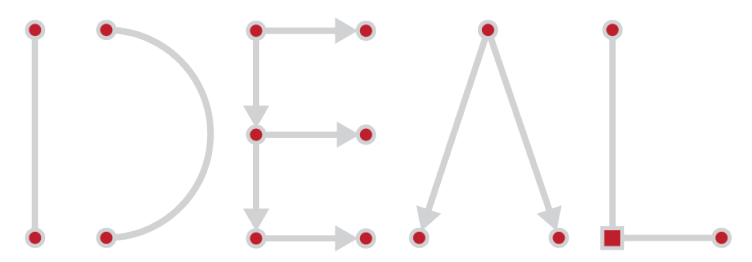
\includegraphics[width=0.6\textwidth]{figures/IDEAL_logo_25.png}
    \end{minipage}%
    \hfill
    \begin{minipage}{0.32\textwidth}
        \centering
        
\includegraphics[width=\textwidth]{figures/eth_logo.pdf}
    \end{minipage}
    \hfill
    \begin{minipage}{0.32\textwidth}
        \centering
        
\includegraphics[width=\textwidth]{figures/manukai_logo.png}
    \end{minipage}
    % End minipage environment

    \vspace{0.5cm}

    \textbf{Swiss Federal Institute of Technology Zurich}\\
    Department of Mechanical and Process Engineering (D-MAVT) \\
    IDEAL – Chair of Artificial Intelligence in Engineering Design \\
    Manukai AG - ETH-Spinoff for AI Manufacturing

    \vspace{1cm}

    \textbf{March 2026}

    Spring Semester 2026

\end{titlepage}

    % Inserts the content of 'titlepage.tex' here, which should define the layout and information for the title page.

    % Roman Page Numbering for Front Matter
    \pagenumbering{roman}
    % Changes page numbering to lowercase Roman numerals (i, ii, iii, ...), typically used for front matter.

    \setcounter{page}{1}
    % Sets the current page number to 1. This is useful to reset page numbering for front matter.

    % Abstract
    \section*{Abstract}
    This semester project investigates parameter-efficient fine-tuning of generative models for Computer-Aided Design (CAD) geometry generation. Specifically, we apply Low-Rank Adaptation (LoRA)---a parameter-efficient method introducing trainable rank decompositions---to the AutoBrep transformer-based model for domain-specific adaptation. We develop a complete pipeline for preprocessing CAD data, fine-tuning with LoRA adapters, and generating novel Boundary Representations. We evaluate training convergence, quantitative metrics, and scalability of LoRA adapters.
    \clearpage
    % \clearpage ensures that the following content starts on a new page.

    % Acknowledgments
    \section*{Acknowledgments}
    I would like to extend my gratitude to my thesis supervisors, Matthew Keeler at the IDEAL lab and Dr. Daniel Wälchli at Manukai AG, for their invaluable guidance, insightful feedback, and continuous support throughout this research. Their expertise in generative modeling and engineering design has significantly shaped the direction and quality of this work.

    \par

    I thank the IDEAL lab team and Manukai AG for providing access to computational resources and data, enabling this research. Special thanks to the research communities working on generative design and parameter-efficient fine-tuning for their foundational contributions to this field.

    \par

    Finally, I am grateful to my colleagues and friends for their encouragement and constructive discussions during the development of this thesis. Their feedback and support were instrumental in bringing this work to completion.
    \clearpage
    % \clearpage ensures that the following content starts on a new page.

    % Table of Contents
    \tableofcontents
    \clearpage
    % Automatically generates the table of contents based on the sections, subsections, etc., in the document.
    % \clearpage ensures that the following content starts on a new page.

    % List of Figures
    \listoffigures
    \addcontentsline{toc}{section}{List of Figures}
    \clearpage
    % Generates a list of all figures included in the document.
    % Adds an entry titled "List of Figures" to the table of contents.
    % \clearpage ensures that the following content starts on a new page.

    % List of Tables
    \listoftables
    \addcontentsline{toc}{section}{List of Tables}
    \clearpage
    % Generates a list of all tables included in the document.
    % Adds an entry titled "List of Tables" to the table of contents.
    % \clearpage ensures that the following content starts on a new page.

    % Abbreviations
    \section*{Abbreviations}
\addcontentsline{toc}{section}{Abbreviations}
\begin{tabular}{p{0.15\textwidth}p{0.85\textwidth}}
	B-Rep & Boundary Representation --- explicit representation of 3D solid surfaces via faces, edges, and vertices \\
	LoRA & Low-Rank Adaptation --- parameter-efficient fine-tuning technique using rank-$r$ decompositions \\
	CAD & Computer-Aided Design --- software tools for designing and modeling engineering geometry \\
	STEP & Standard for the Exchange of Product Model Data --- ISO 10303 file format for CAD models \\
	UV-Grid & 2D parametric coordinate system on a B-Rep face surface \\
	AutoBrep & State-of-the-art transformer-based generative model for B-Rep synthesis \\
	NURBS & Non-Uniform Rational B-Splines --- parametric surface/curve representation standard in CAD \\
	VAE & Variational Autoencoder --- generative model learning compressed latent representations \\
	GNN & Graph Neural Network --- neural architecture operating on graph-structured data \\
	W\&B & Weights \& Biases --- ML experiment tracking and visualization platform \\
\end{tabular}

    \clearpage
    % Inserts the content of 'abbreviations.tex' here, which should contain a list of abbreviations used in the document.
    % \clearpage ensures that the following content starts on a new page.

    % Start Arabic Page Numbering
    \pagenumbering{arabic}
    % Changes page numbering to Arabic numerals (1, 2, 3, ...), typically used for the main body of the document.

    \pagestyle{main}
    % Sets the page style to 'main', which is defined in 'plusstyle.sty'.
    % This usually includes customized headers and footers.

    % Chapters
    \section{Introduction}
\label{chap:introduction}

%===============================================================
\subsection{Context and Motivation}
%===============================================================

The idea for this thesis came from the ETH spinoff Manukai AG where they need synthetic CAD training data for their machine learning models for CAM manufacturing. Currently they do this using heuristics, generating random sequences of extrusions. Additionally they need to finetune their models on small customer CAD datasets. The companies dont want to share their propietary CAD data beyond their personal applications, as it might contain trade secrets, so Manukai needs to finetune their models with very limited data each time anew to avoid leakage between companies. Here it would be very useful to be able to generate similar high-quality data, which is where this project comes in.

The initial Idea of using a diffusion model following BrepGen \cite{Xu2024brepgen} was postponed as for two main reasons. Firstly, in between the first discussion of the project and the start, another student at Manukai had already explored BrepGen \cite{Xu2024brepgen} and did not come to useful results. Secondly, a new paper was published by the main author of this paper, called AutoBrep \cite{Xu2025autobrep}, which had more promising results. It generated B-Rep's with higher quality and higher complexity Fig \ref{fig:validity} which could be reproduced during inference aswell.

\begin{figure}[h!]
	\centering
	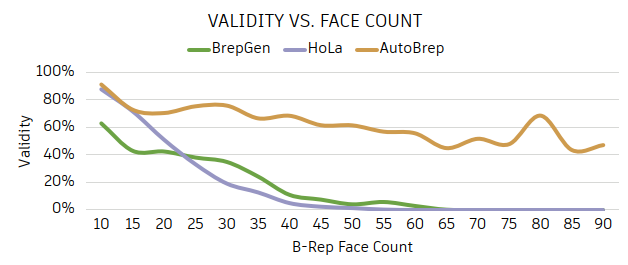
\includegraphics[width=0.6\textwidth]{figures/validity.png}
	\caption{Training and Validation Loss Over Epochs}
	\label{fig:validity}
\end{figure}


%===============================================================
\subsection{Problem Statement}
%===============================================================

Machine learning models for CAD geometry generation have been developed, including the state-of-the-art AutoBrep model, which uses transformer-based architectures to generate Boundary Representations (B-Reps) autoregressively. However, applying such models to new, specialized design domains presents significant challenges:

\par

\textbf{Key challenges:}
\begin{itemize}
    \item \textbf{Domain Adaptation}: Pre-trained models reflect patterns from their training data; specialized design domains (e.g., specific mechanical parts, architectural elements) may have unique characteristics not well-represented in general training corpora
    \item \textbf{Limited Data}: High quality CAD data which is B-Rep compatible is scarce and expensive. It exists in large quantities in industrial companies, but often as parts of trade secrets, and is created in work-intensive manual work by experts.
\end{itemize}

%===============================================================
\subsection{Thesis Objective}
%===============================================================

This work addresses these challenges by investigating \textit{parameter-efficient fine-tuning} of generative CAD models using Low-Rank Adaptation (LoRA). The core research question is:

\par

\textbf{``Can large pre-trained generative CAD models like AutoBrep from \cite{Xu2025autobrep} be efficiently adapted to specialized design domains with limited data using Low Rank Adaptation?''}

To answer this, we:
\begin{enumerate}
    \item Implement a complete pipeline for LoRA-based fine-tuning of the AutoBrep model
    \item Demonstrate domain-specific adaptation on custom CAD datasets
    \item Analyze scalability of multiple LoRA adapters for different domains
    \item Evaluate practical utility and limitations of the approach
\end{enumerate}

%===============================================================
\subsection{Contributions}
%===============================================================

This thesis makes the following contributions to the field of generative design and machine learning for CAD:

\par

\begin{enumerate}
    \item \textbf{Practical Framework}: An end-to-end implementation of LoRA fine-tuning for AutoBrep, including data preprocessing, training, and inference pipelines

    \item \textbf{Efficiency Analysis}: Empirical demonstration whether domain-specific performance can be achieved with only $\approx$1\% additional trainable parameters and order of 500 samples, enabling fine-tuning with very limited data and without changing the base model's parameters

    \item \textbf{Reproducibility}: Detailed documentation of hyperparameters, code, training curves and experimental procedures enabling future research and practical adoption
\end{enumerate}

%===============================================================
\subsection{Thesis Structure}
%===============================================================

The remainder of this thesis is organized as follows:

\begin{itemize}
    \item \textbf{Chapter~\ref{chap:background}}: Background and related work on B-Reps, generative models for CAD, LoRA, and related domain adaptation techniques

    \item \textbf{Chapter~\ref{chap:methodology}}: Detailed methodology covering AutoBrep architecture, LoRA integration, data preprocessing, and training procedures

    \item \textbf{Chapter~\ref{chap:results}}: Experimental results including training convergence, quantitative evaluation, and qualitative analysis of generated models

    \item \textbf{Chapter~\ref{chap:discussion}}: Discussion of findings, limitations, and directions for future research

    \item \textbf{Chapter~\ref{chap:conclusion}}: Summary of contributions and practical implications
\end{itemize}

    % Chapter 1: Introduction - Problem statement, context, and thesis objectives

    \section{Background and Related Work}
\label{chap:background}

%===============================================================
\subsection{B-Representation (B-Rep) Fundamentals}
%===============================================================

The Boundary Representation (B-Rep) is a fundamental data structure in Computer-Aided Design (CAD) systems. B-Reps describe 3D solid objects by explicitly representing their boundary surfaces. This representation form enables precise geometric modeling and is widely used in industrial design, mechanical engineering, and manufacturing.
The key components of a B-Rep include faces, edges, and vertices, along with their topological relationships.

\par

\textbf{Key characteristics of B-Reps:}
\begin{itemize}
	\item \textbf{Explicit Surface Representation}: Surfaces are defined using parametric equations (e.g., Non-Uniform Rational Basis Splines)
	\item \textbf{Topological Consistency}: Maintains relationships between geometric elements
	\item \textbf{Industry Standard}: Widely supported by professional CAD software (Autodesk, Solidworks, FreeCAD)
	\item \textbf{High Precision}: Suitable for manufacturing and detailed design specifications
\end{itemize}

%===============================================================
\subsection{Generative Models for CAD}
%===============================================================

Recent advances in deep learning have enabled the development of neural models capable of generating CAD geometry. Two complementary approaches have emerged: diffusion-based and autoregressive methods, each with distinct advantages for direct B-Rep synthesis.

\par

\textbf{Generative modeling approaches:}
\begin{itemize}
	\item \textbf{Autoregressive Models}: Generate sequences token-by-token, capturing dependencies
	\item \textbf{Diffusion Models}: Iteratively refine from noise, offering excellent quality
	\item \textbf{VAE-based Methods}: Learning compressed latent representations
	\item \textbf{Hybrid Approaches}: Combining multiple techniques for optimal performance
\end{itemize}

%===============================================================
\subsubsection{BrepGen: Diffusion-Based Approach}
%===============================================================

\cite{Xu2024brepgen} introduces BrepGen, a diffusion-based model for direct B-Rep generation. The key innovation is a \textit{structured latent geometry} representation that encodes B-Reps as hierarchical trees with three levels: faces, edges, and vertices.

\begin{figure}[h!]
	\centering
	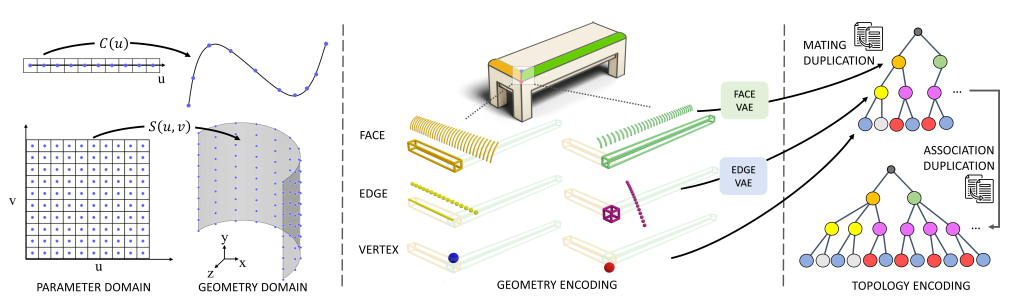
\includegraphics[width=1\textwidth]{figures/brepgen_encoding.png}
	\caption{Encoding B-rep's into point clouds: 32 x 32 points are sampled over each surface and 32 points over each edge of the solid. The faces and edges are then stored in a hierarchical tree which encodes the topology (connections between different faces and edges)}
	\label{fig:brepgen_encoding}
\end{figure}
\begin{figure}[h!]
	\centering
	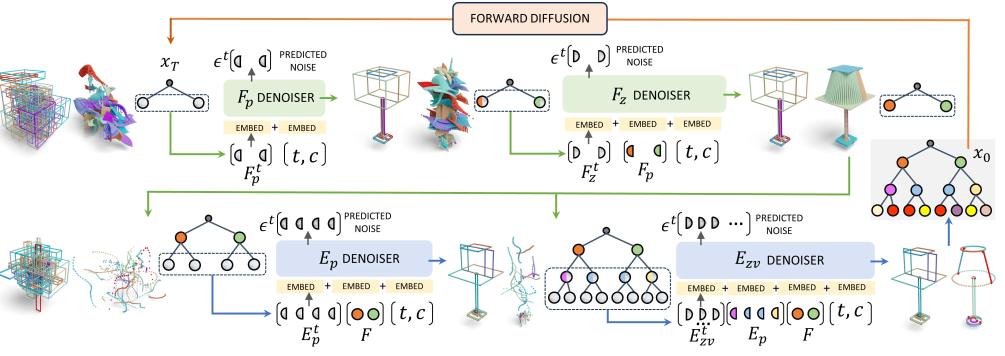
\includegraphics[width=1\textwidth]{figures/brepgen_model.png}
	\caption{Generating new B-rep's: The noise for faces and bounding boxes (spacial lmitis of the faces) is denoised with two denoisers. Conditioned on these faces, edge noise and bounding boxes are generated and again twice denoised}
	\label{fig:brepgen_model}
\end{figure}

 Postprocessing: The generated edge and and face pointclouds are sewed back into  B-rep's in .step format using the Open-Cascade library.



%===============================================================
\subsubsection{AutoBrep: Autoregressive Approach}
%===============================================================

\cite{Xu2025autobrep} presents AutoBrep, an autoregressive Transformer that unifies B-Rep geometry and topology into a single stream of discrete tokens. Unlike multi-stage diffusion, AutoBrep generates B-Reps end-to-end via next-token prediction Fig. \ref{fig:scheme}.

\begin{figure}[h!]
	\centering
	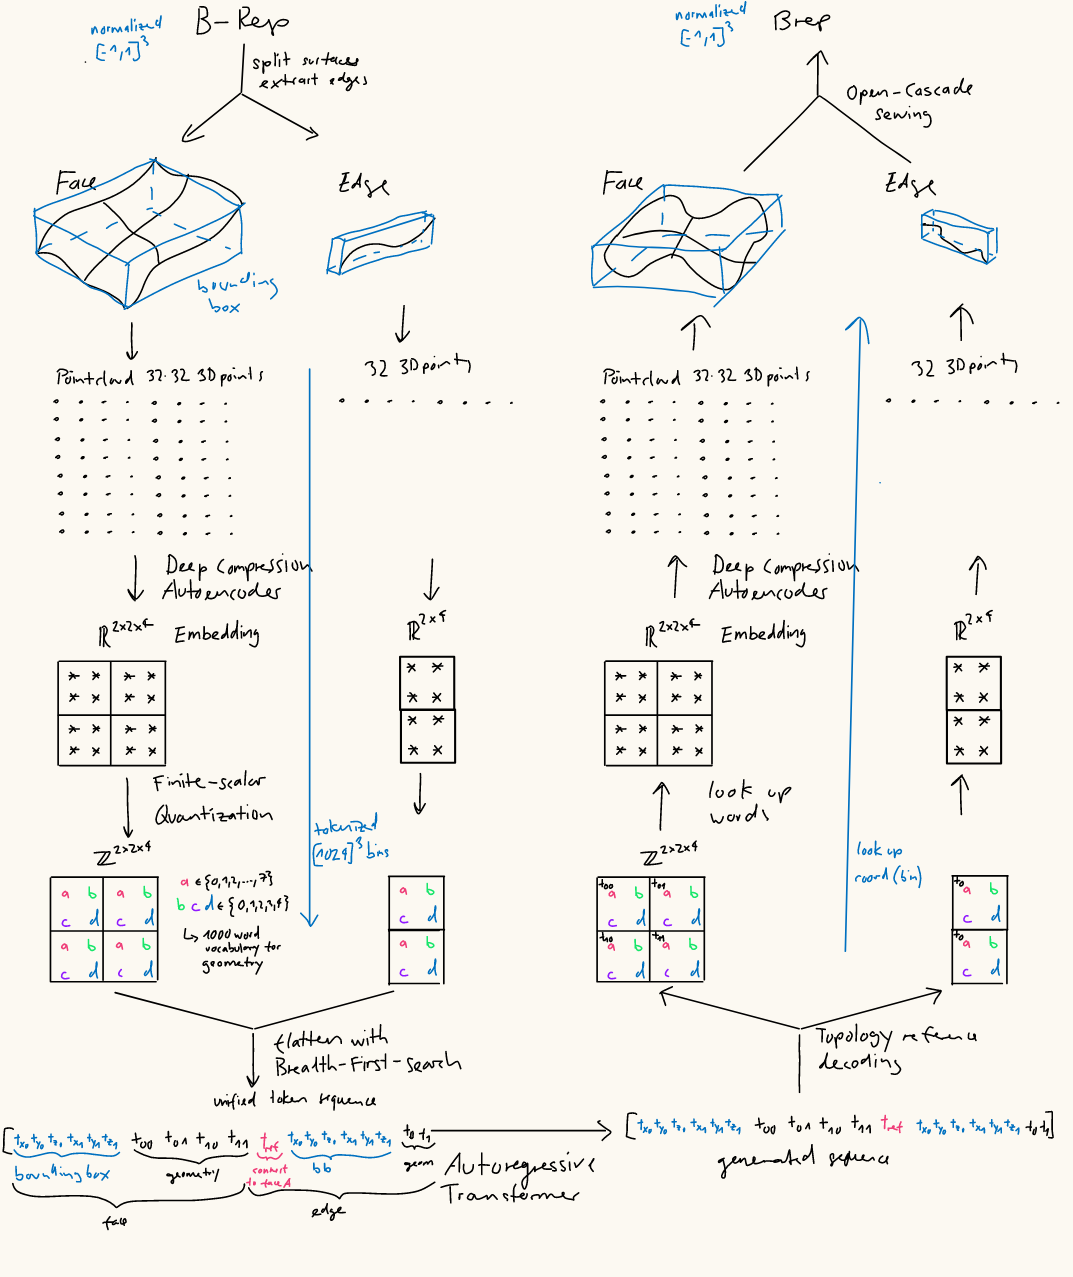
\includegraphics[width=1\textwidth]{figures/autobrep_scheme.png}
	\caption{Starting from the top left, the encoding into point clouds is equivalent to BrepGen. Next, the faces are encoded into Tokens using a VAE and quantized with finite scalar quantization into a 1000 word vocabulary. Tokens are then places in a sequence where the order is retrieved from a Breadth-First-Search over the surfaces and edges of the B-Rep. This sequence is then fed into a GPT-like transformer model using a causal mask. Then the transformer predicts the sequence (during training, else a new sequence) through next-token prediction and the process repeats in the opposite direction.}
	\label{fig:scheme}
\end{figure}

\par


Key advantages: (1) Single unified architecture vs. multi-stage pipeline, (2) 2--5$\times$ faster inference via next-token prediction, (3) Native support for B-Rep completion through next token prediction, (4) Scalability to 100+ face solids.

\par

\textbf{Comparison:}
\begin{itemize}
	\item \textbf{BrepGen}: Six modules (2 VAEs + 4 diffusion denoisers), multi-stage cascading, slower (~10 sec/sample), supports conditional generation
	\item \textbf{AutoBrep}: Three modules (2 autoencoders + 1 transformer), unified pipeline, faster (~0.46 sec/sample), natively supports autocompletion with face preservation
\end{itemize}

%===============================================================
\subsection{Low-Rank Adaptation (LoRA)}
%===============================================================

LoRA (Low-Rank Adaptation) is a parameter-efficient fine-tuning technique introduced by \cite{Hu2021lora}. Rather than fine-tuning all model parameters, LoRA introduces small trainable low-rank decompositions in the projection matrices of attention layers within a Transformer. This approach dramatically reduces memory requirements and training time while maintaining competitive or superior performance relative to full fine-tuning.

\par

\textbf{Core Mechanism:}

The fundamental idea is to decompose weight updates as a product of two low-rank matrices:
\[
W' = W_0 + \Delta W = W_0 + AB^T
\]
where $W_0 \in \mathbb{R}^{d_{\text{out}} \times d_{\text{in}}}$ is the frozen pre-trained weight matrix, $A \in \mathbb{R}^{d_{\text{out}} \times r}$, $B \in \mathbb{R}^{d_{\text{in}} \times r}$, and $r \ll d_{\text{in}}, d_{\text{out}}$ (rank) is a small hyperparameter. During fine-tuning, only $A$ and $B$ are trainable, while $W_0$ remains frozen.

\par

This approach is very compute and memory efficient by only adding adapters of around 1\% model size to the base model without modifying it.

\begin{figure}[h]
	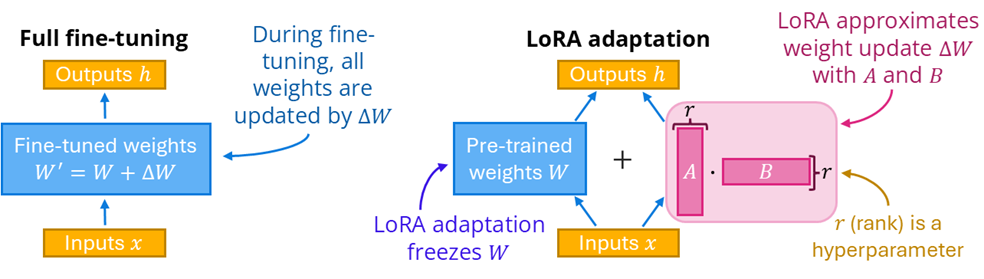
\includegraphics[width=0.76\textwidth]{figures/lora.png}
	\centering
	\caption{LoRA adapters are added in the attention layers to the query and valuey weight matrices \cite{Hu2021lora}.}

	\label{fig:lora}
\end{figure}

%===============================================================
\subsection{Related Work in Generative Design}
%===============================================================

The field of neural CAD generation has grown rapidly in recent years. Multiple approaches have been explored:

\begin{itemize}
	\item \textbf{CAD Agents}: Copilot the CAD software with a human in the loop
	\item \textbf{Graph Neural Networks}: Capturing the topological structure of CAD models through graphs
	\item \textbf{Transformer-based Methods}: Leveraging attention mechanisms for long-range dependencies
	\item \textbf{Multi-modal Learning}: Combining text, images, and geometry for conditional generation
\end{itemize}

The integration of LoRA with pre-trained generative models enables efficient adaptation to specialized domains without requiring large labeled datasets or extensive computational resources. This is particularly valuable for downstream applications where domain-specific data is limited.

    % Chapter 2: Background and Related Work - B-Reps, generative models, LoRA, related work

    \section{Methodology}
\label{chap:methodology}

%===============================================================
\subsection{AutoBrep Transformer Architecture}
%===============================================================

AutoBrep is a decoder-only transformer model with approximately 1 billion parameters, designed for autoregressive generation of Boundary Representations (B-Reps). The architecture consists of:

\begin{itemize}
	\item \textbf{35-layer Transformer decoder} with embedding dimension $d = 768$
	\item \textbf{Multi-head attention}: Processes query (\texttt{to\_q}), key, and value (\texttt{to\_v}) projection layers
	\item \textbf{Position-wise feedforward networks (MLP)}: Projections $768 \to 16384 \to 768$
	\item \textbf{Tokenization layers}: Meta tokens (complexity class), CAD tokens (face/edge/topology sequences), and geometry tokens
\end{itemize}

The model is trained on approximately 1 million B-Reps and achieves reported validity rates up to 50\% for complex geometries (up to 100 faces). It operates autoregressively, predicting the next token conditioned on all preceding tokens in the sequence.

%===============================================================
\subsection{LoRA Fine-tuning Configuration}
%===============================================================

Following the LoRA approach described in Chapter~\ref{chap:background}, we apply low-rank adapters to the AutoBrep transformer architecture. Rather than full fine-tuning, only adapter parameters are trainable while the 1B-parameter base model remains frozen.

\textbf{Adapter Placement and Dimensions:}

\[
\mathbf{z}_q = \mathbf{W}_q \cdot \mathbf{x} + \frac{\alpha}{r} \cdot \mathbf{x} \cdot \mathbf{B} \cdot \mathbf{A}
\]
where $\mathbf{A} \in \mathbb{R}^{r \times 768}$, $\mathbf{B} \in \mathbb{R}^{768 \times r}$.

AutoBrep is a 35-layer decoder-only Transformer with embedding dimension $d = 768$. We explored two adapter placement strategies:

\begin{enumerate}
	\item \textbf{Attention-Only} (Primary): Adapters inserted into query (\texttt{to\_q}) and value (\texttt{to\_v}) projection layers:

	\item \textbf{Attention + Feedforward} (Ablation): Additional adapters on the feedforward projection layers $\text{ff}: \mathbb{R}^{768} \to \mathbb{R}^{16384}$ to capture more model capacity.
\end{enumerate}


Each adapter pair at rank $r$ contributes trainable parameters. We explored two configurations:

\textbf{Attention-Only Configuration:} Across 35 layers with 2 adapters per layer ($35 \times 2 = 70$ total), with $d=768$. 

\textbf{Attention + Feedforward Configuration:} Additionally inserting adapters into the feedforward projections ($768 \to 16384 \to 768$) adds substantial capacity.

Across 35 layers: $\text{Extra} = 35 \times 17,152 \times r = 600,320 \times r$ parameters.

\begin{table}[h!]
	\centering
	\caption{LoRA Parameter Efficiency: Attention-Only vs. Attention + Feedforward}
	\label{tab:lora_params}
	\small
	\begin{tabularx}{\textwidth}{l >{\centering\arraybackslash}X >{\centering\arraybackslash}X >{\centering\arraybackslash}X}
		\toprule
		\textbf{Config} & \textbf{Rank ($r$)} & \textbf{Params (M)} & \textbf{\% Base} \\
		\midrule
		\multirow{4}{*}{\textbf{Attention}} & 4 & 0.43 & 0.043\% \\
		& 8 & 0.86 & 0.086\% \\
		& 16 & 1.72 & 0.172\% \\
		& 32 & 3.44 & 0.344\% \\
		\midrule
		\multirow{2}{*}{\textbf{Attention + FF}} & 16 & 12.12 & 1.212\% \\
		& 32 & 24.24 & 2.424\% \\
		\bottomrule
	\end{tabularx}
\end{table}

Even with feedforward adapters at $r=32$, total parameters remain $<2.5\%$, but at significant cost in memory and training time. Attention-only adapters achieved comparable results with minimal overhead.


%===============================================================
\subsection{Data Preparation Pipeline}
%===============================================================

A custom data processing pipeline converts raw STEP files (Fig.~\ref{fig:raw}) into a structured parquet dataset compatible with AutoBrep tokenization:

\par

\textbf{Processing steps:}
\begin{enumerate}
	\item \textbf{STEP Loading and Feature Extraction}: Parse CAD solids using Open Cascade, extracting faces, edges, and topology information
	\item \textbf{UV-Grid Sampling}: Sample UV-parameter spaces to create dense point clouds representing geometric surfaces 
	\item \textbf{Geometry Normalization}: Normalize coordinates to the $[-1, 1]^3$ range bounding box (Fig.~\ref{fig:preprocessed})
	\item \textbf{Serialization}: Convert numpy arrays to bytes for compact storage in the dataset
	\item \textbf{Parquet Export}: Write preprocessed geometries with corresponding bounding boxes, complexity metadata (face count), and split into train/validation (0.9/0.1) splits
\end{enumerate}

The resulting parquet dataset contains serialized geometry tensors (faces, edges) with corresponding bounding box annotations and topology metadata.

\begin{figure}[h!]
	\centering
	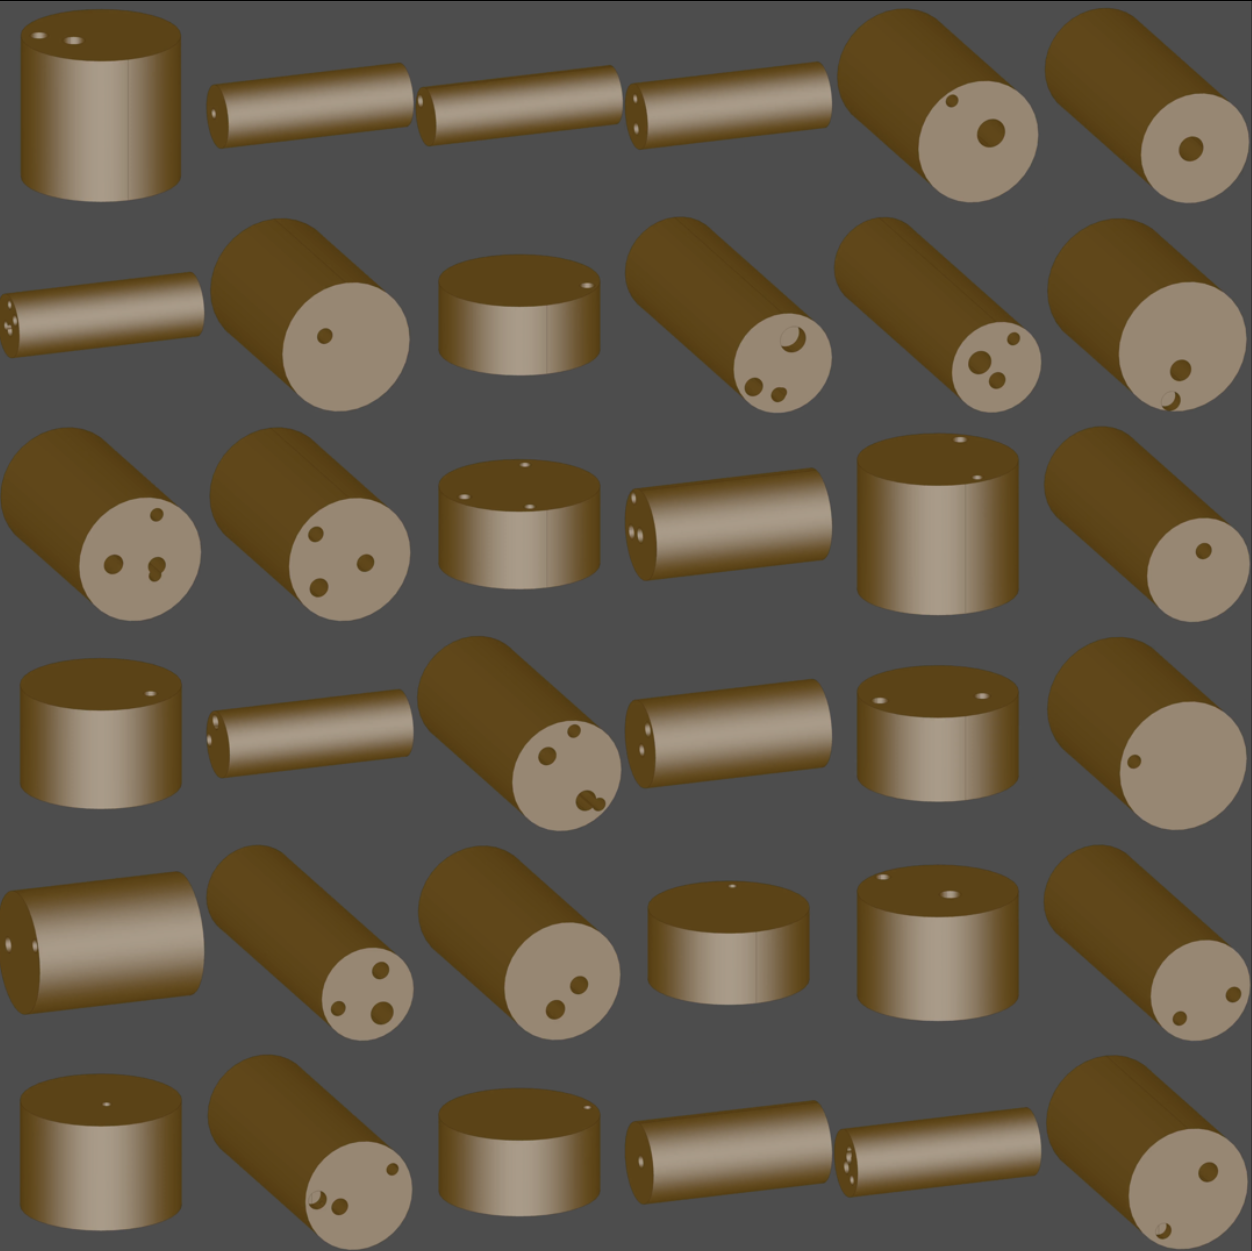
\includegraphics[width=0.5\textwidth]{figures/step_train.png}
	\caption{Raw .step file renderings of the generic cylinders with holes dataset provided by Manukai}
	\label{fig:raw}
\end{figure}

\begin{figure}[h!]
	\centering
	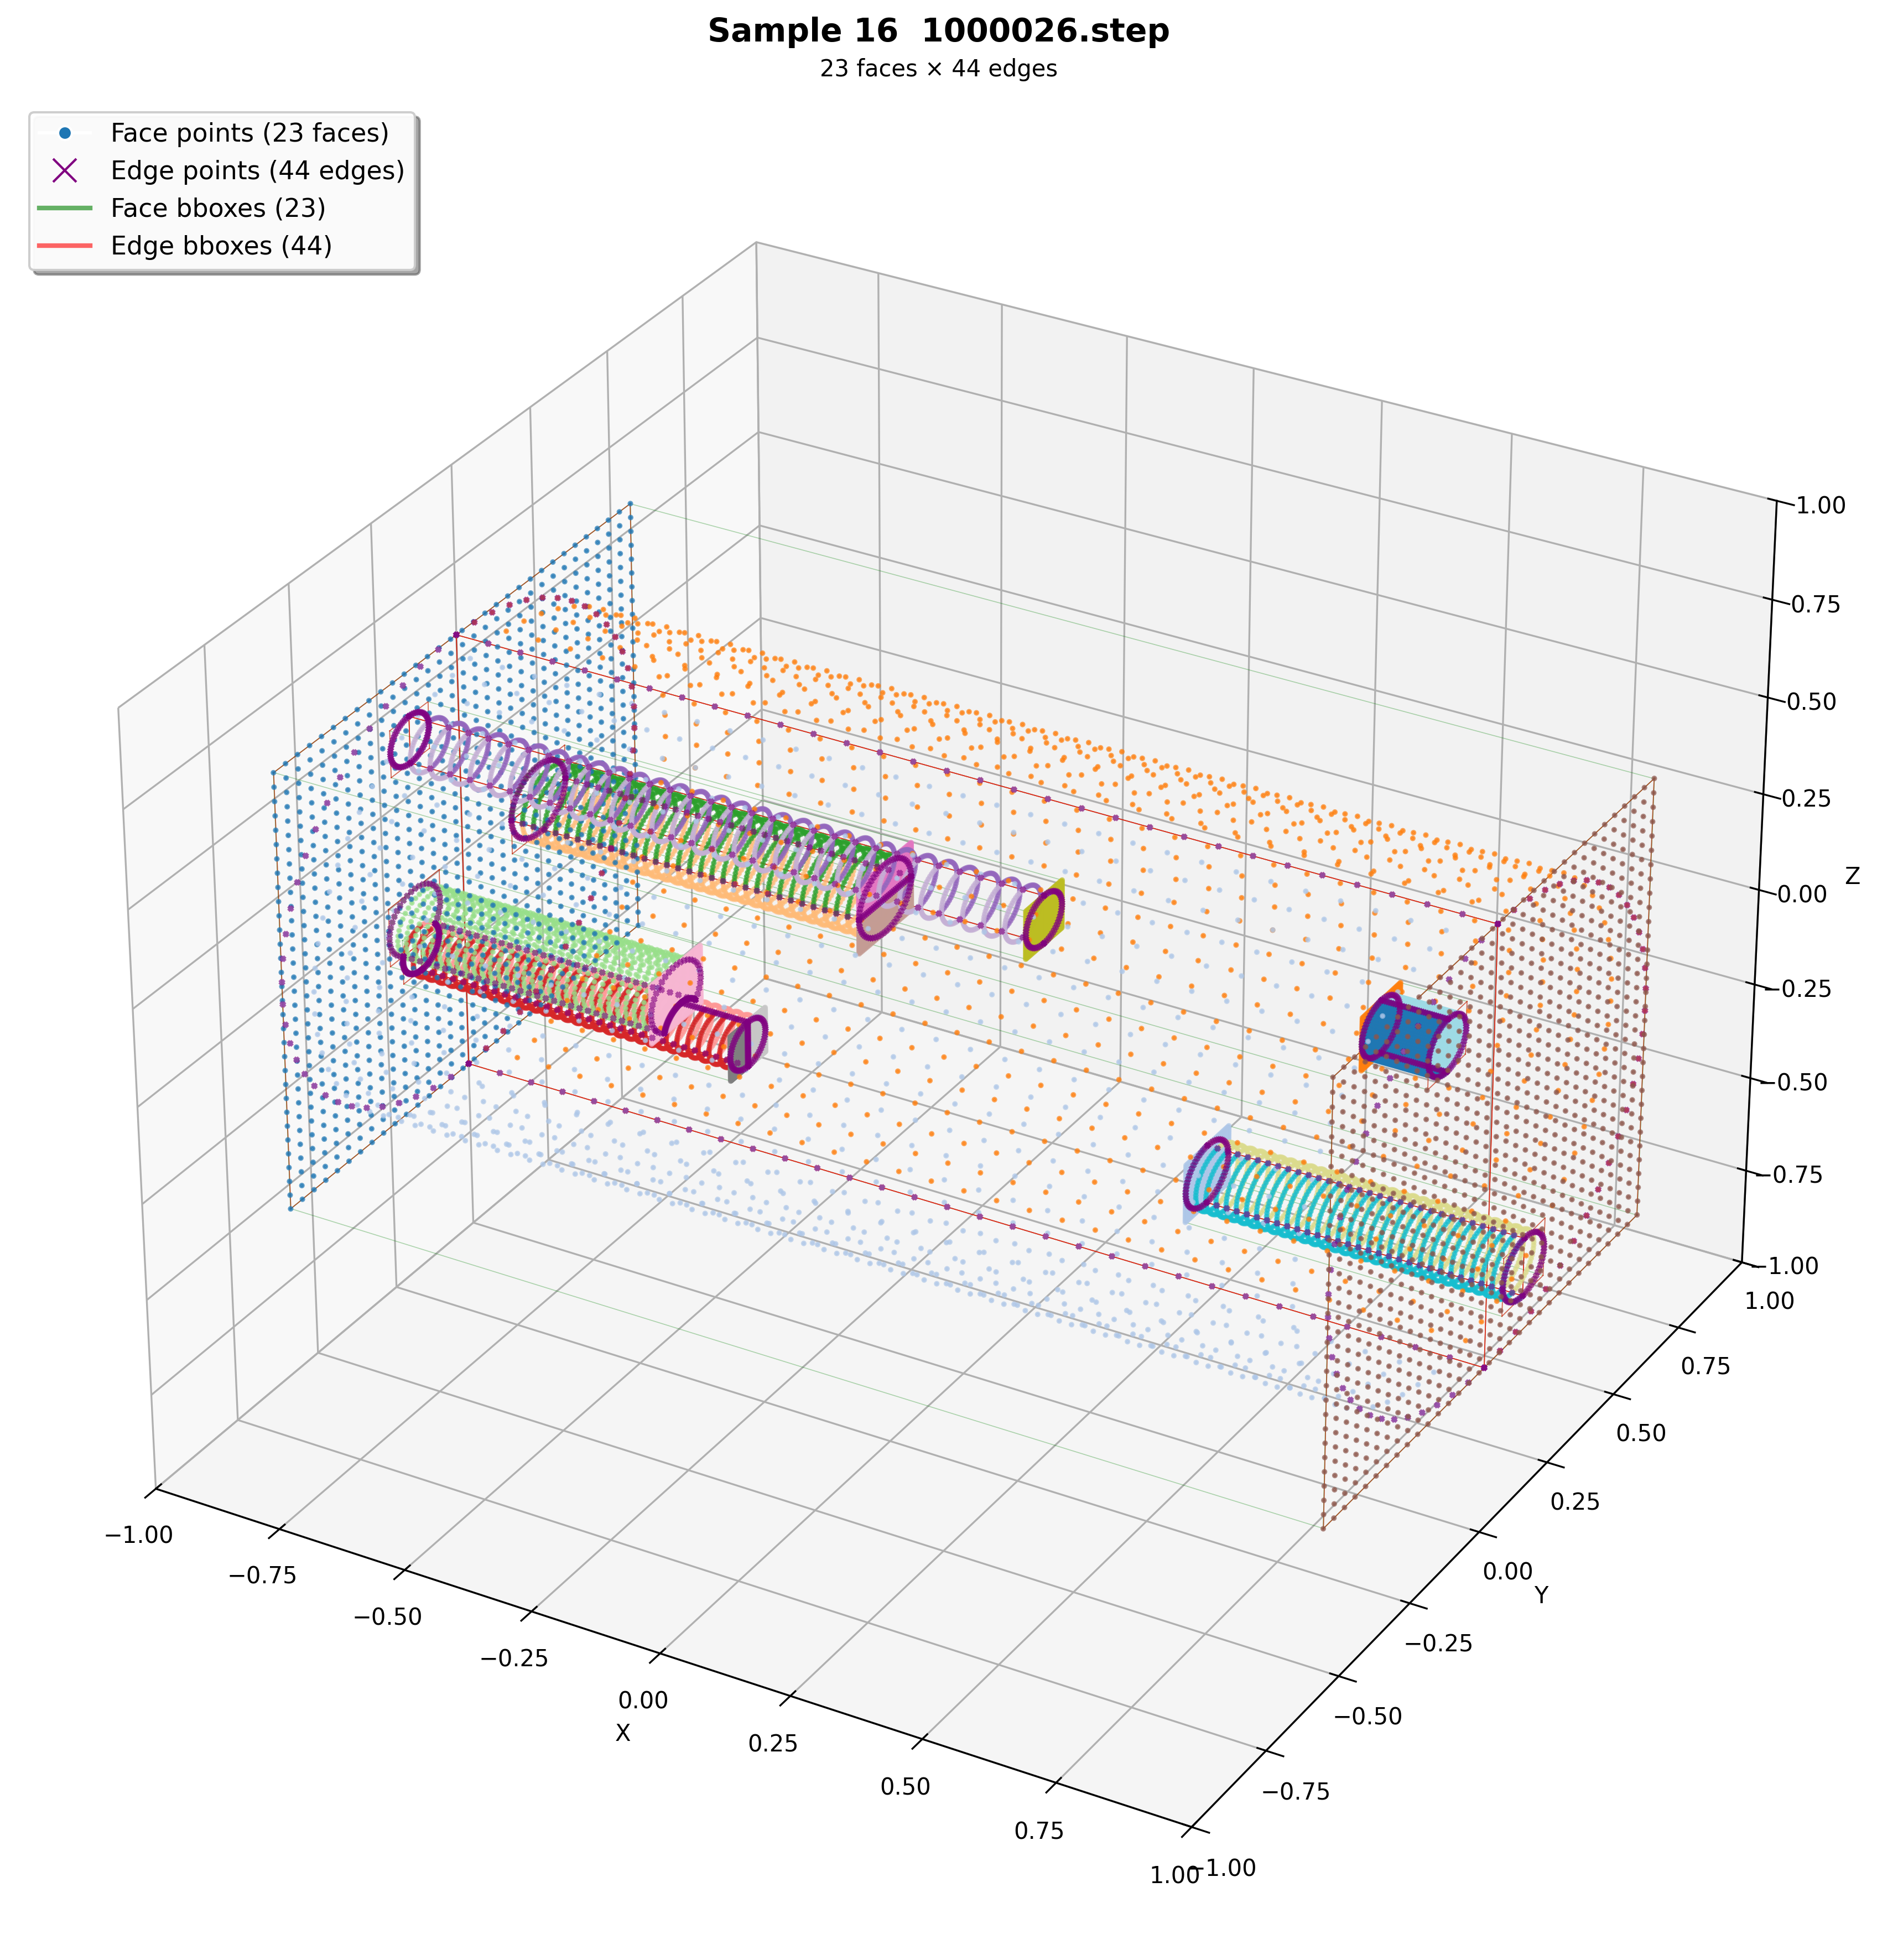
\includegraphics[width=0.5\textwidth]{figures/parquet_sample_016.png}
	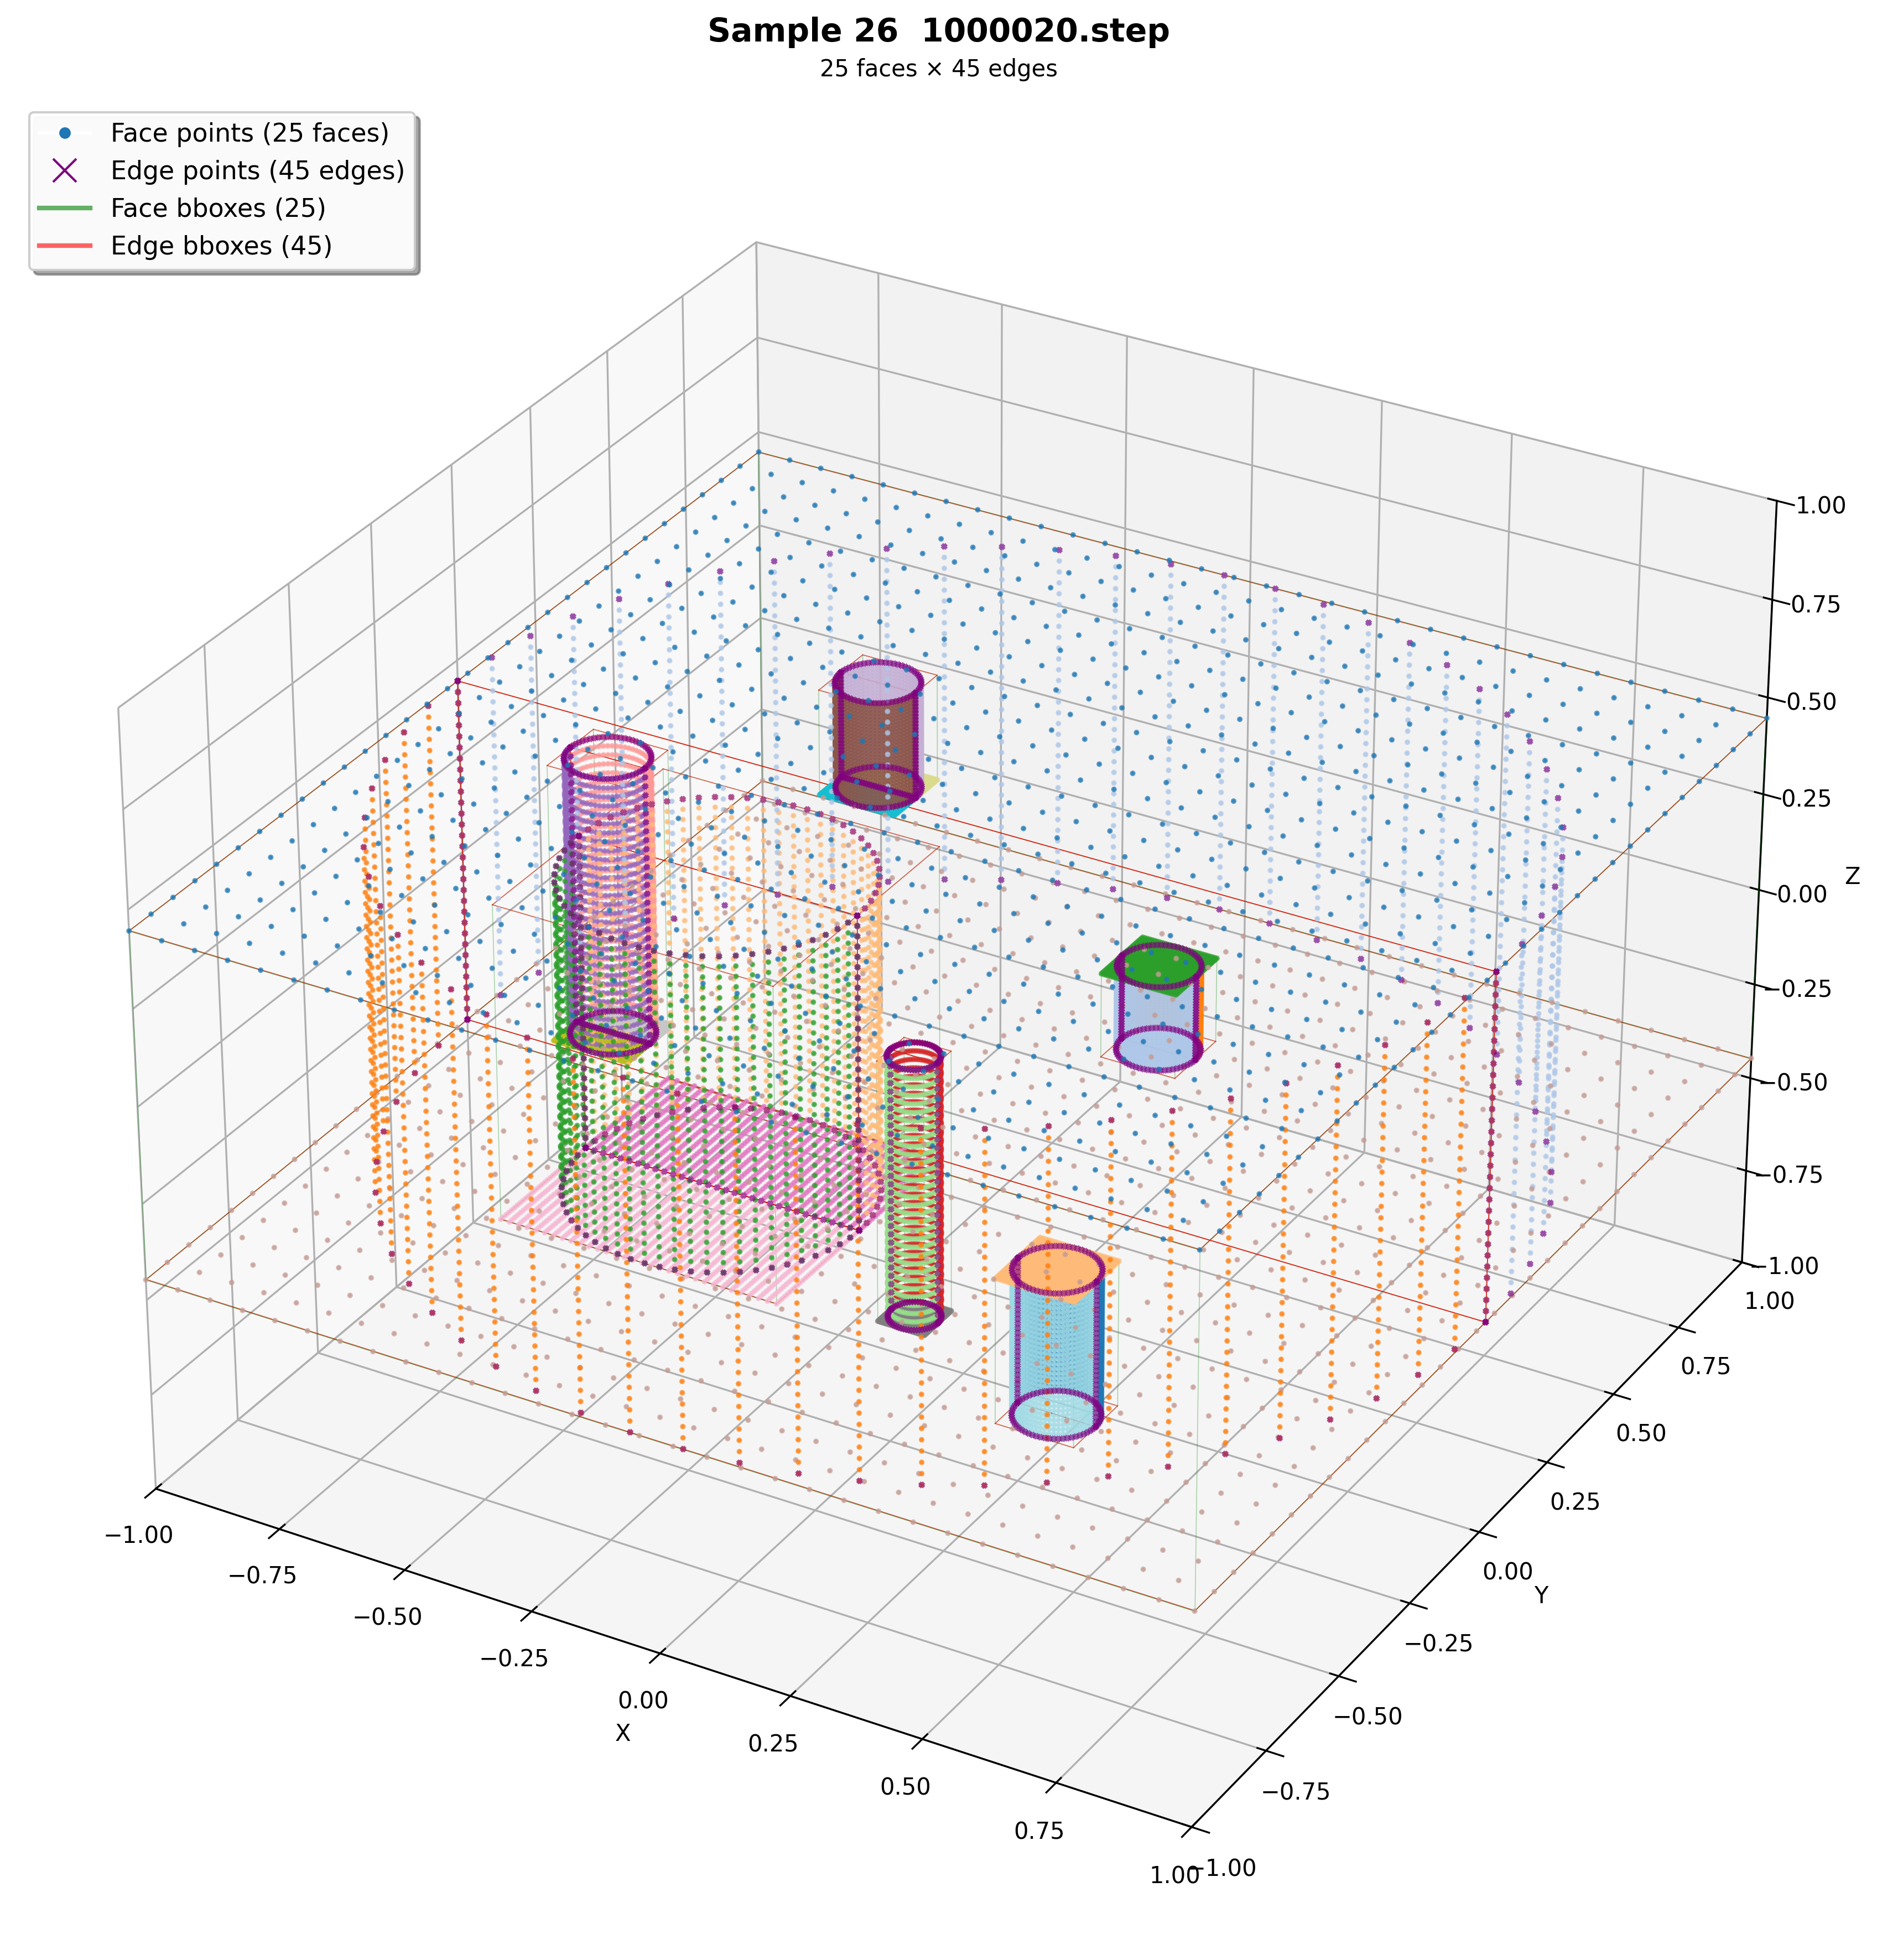
\includegraphics[width=0.49\textwidth]{figures/parquet_sample_026.png}
	\caption{Two examples of preprocessed point cloud solids of the generic cylinders with holes}
	\label{fig:preprocessed}
\end{figure}

\newpage

%===============================================================
\subsection{Training Setup}
%===============================================================

Fine-tuning is performed using the AdamW optimizer on the frozen base model with LoRA adapters as the only trainable parameters. Hyperparameter selection in table \ref{tab:training_hyperparams} follows established LoRA fine-tuning practices \cite{Hu2021lora, UnSloth2024lora}.
\par

\begin{table}[h!]
	\centering
	\caption{Training Hyperparameters following \cite{Hu2021lora}}
	\label{tab:training_hyperparams}
	\small
	\begin{tabularx}{\textwidth}{@{}l X l@{}}
		\toprule
		\textbf{Parameter} & \textbf{Value} & \textbf{Notes} \\
		\midrule
		Batch Size & 4 & Same as in Autobrep \cite{Xu2025autobrep} \\
		Number of Epochs & 4 & Typical  \\
		Learning Rate & 1e-4 to 5e-5 & Lower rates recommended for small datasets to prevent overfitting \\
		LoRA Rank & 8--32 & Balance between model capacity and parameter efficiency \\
		LoRA Alpha & $\approx 4 \times$ r & Effective scaling = $\alpha / r$; adjust for sensitivity \\
		Optimizer & AdamW & Standard choice with weight decay for regularization \\
		\bottomrule
	\end{tabularx}
\end{table}

\par

\textbf{GPU Memory Optimization:} Training on a single RTX 4090 GPU (24 GB) was enabled through three techniques: (1) casting the model to bfloat16 precision to reduce memory overhead, (2) using PyTorch's expandable memory segments
\newline (\texttt{PYTORCH\_ALLOC\_CONF=expandable\_segments:True}) to avoid fragmentation, and (3) periodic GPU cache cleanup (\texttt{torch.cuda.empty\_cache()}) every 10 batches. These techniques allowed efficient training without requiring gradient accumulation.

\par

The train and validation loss function is computed using cross-entropy loss from the AutoBrep module, which measures the divergence between predicted and ground-truth token distributions.

Training is monitored via Weights \& Biases (W\&B) for real-time loss tracking, learning rate schedules, and system metrics.

%===============================================================
\subsection{Inference and B-Rep Generation}
%===============================================================

During inference, the fine-tuned model generates B-Rep sequences autoregressively, conditioned on a complexity token. Generation is controlled via temperature sampling; top-$p$ (nucleus) sampling is kept constant at 0.95 to ensure diverse yet reasonable outputs. During training unconditional samples are created after each epoch.
Token sequences are decoded into geometric primitives (surfaces, curves) and topological relationships via the FSQ-VAE decoders. The reconstructed B-Rep geometry is then validated and assembled into watertight solids (STEP files) using the AutoBrepBuilder with the following parameters:

\begin{table}[h!]
	\centering
	\caption{Inference and B-Rep Reconstruction Parameters}
	\label{tab:reconstruction_tolerances}
	\small
	\begin{tabularx}{\textwidth}{@{}l l l@{}}
		\toprule
		\textbf{Parameter} & \textbf{Value} & \textbf{Interpretation} \\
		\midrule
		\multicolumn{3}{l}{\textit{Inference Control}} \\
		\midrule
		Complexity Token & 14--17 & 14: $<$25 faces, 15: $<$50 faces, 16: $>$50 faces, 17: random \\
		Temperature & 0.3--0.8 & Controls sampling diversity; 0.5--0.7 found optimal for fidelity+diversity \\
		\midrule
		\multicolumn{3}{l}{\textit{Reconstruction Tolerances}} \\
		\midrule
		Sewing Tolerance & $2 \times 10^{-3}$ & Max distance for edge-face sewing (watertightness) \\
		Vertex Threshold & $2 \times 10^{-3}$ & Max separation for vertex merging \\
		Z-Threshold & 0 & Z-coordinate deviation check enforced to zero (strict) \\
		\bottomrule
	\end{tabularx}
\end{table}

A B-Rep is considered valid if it passes the solid modeling kernel's validation checks: all edges are shared by exactly 2 faces (no dangling edges) and the topology forms a closed manifold (watertight) within tolerances.

    % Chapter 3: Methodology - AutoBrep architecture, LoRA integration, data pipeline, training setup

    \section{Experimental Results}
\label{chap:results}

%===============================================================
\subsection{Baseline Inference}
%===============================================================

In Fig.~\ref{fig:untuned_samples} we can see that the unmodified AutoBrep model indeed generates impressive B-Rep's with high complexity and apparent correctness. Each of these STEP samples were rendered from various angles and concatenated in a GIF showing them from all directions for inspection.

\begin{figure}[h!]
	\centering
	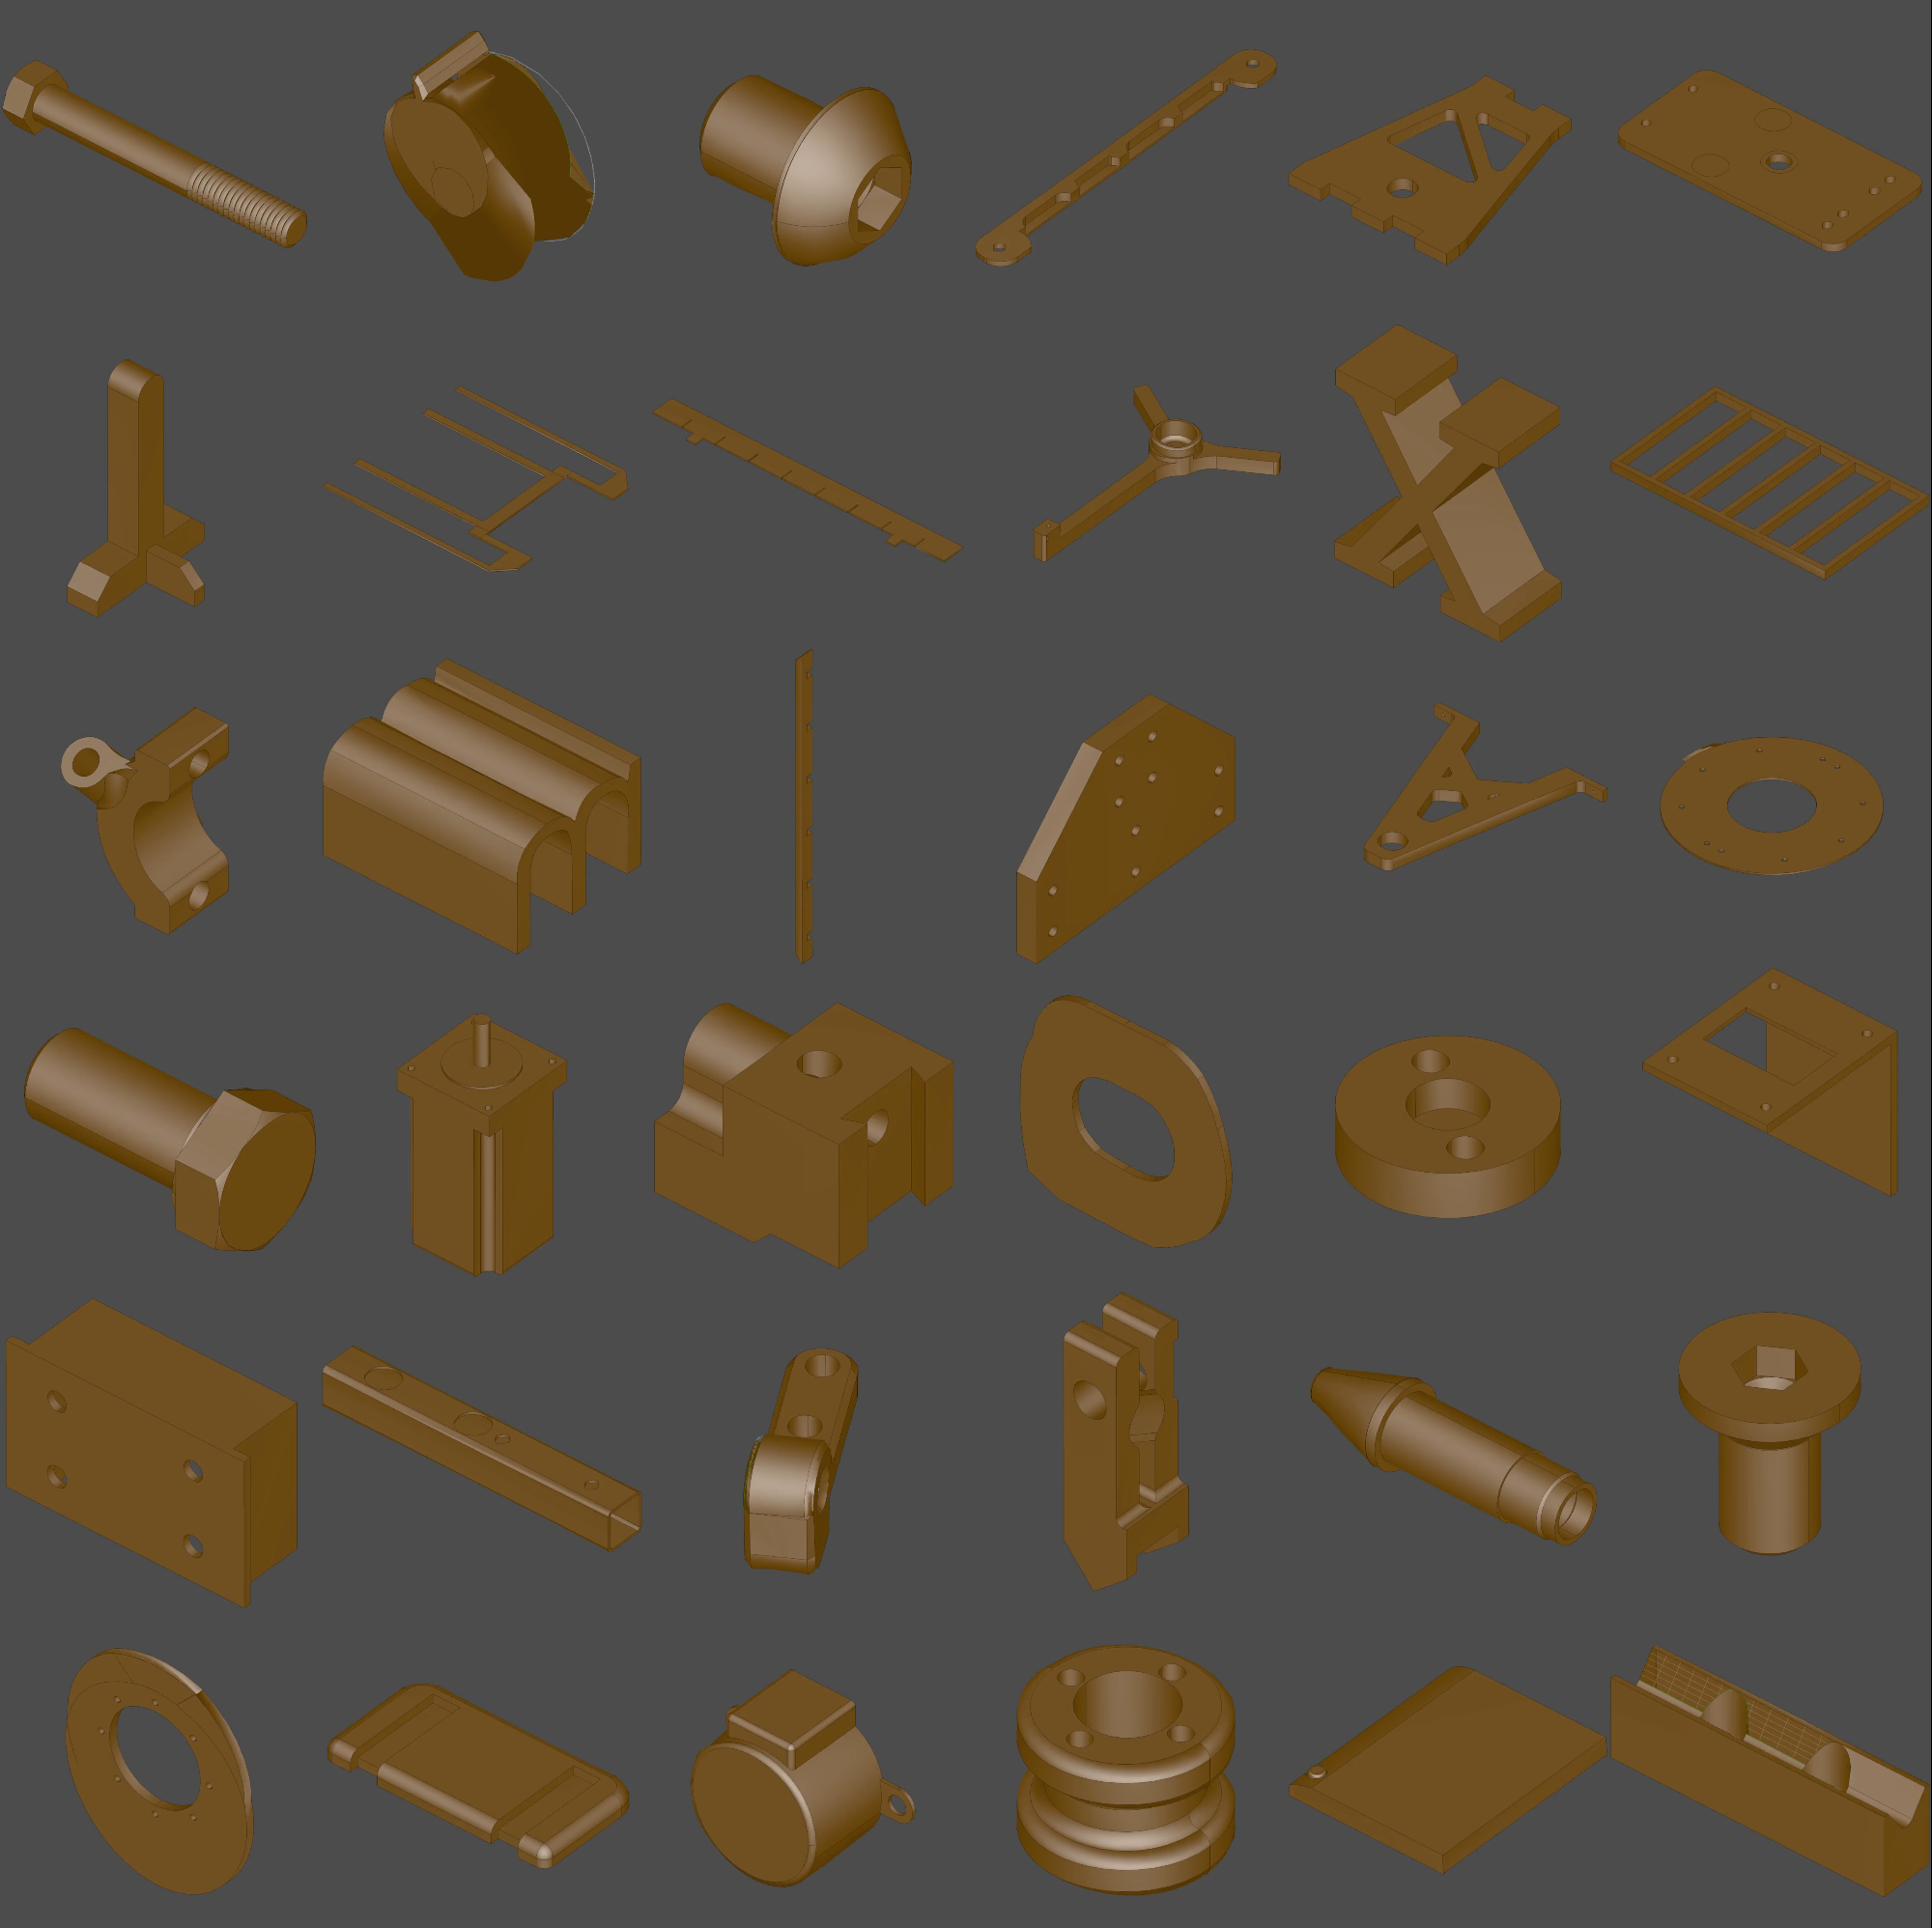
\includegraphics[width=0.66\textwidth]{figures/untuned_medium.png}
	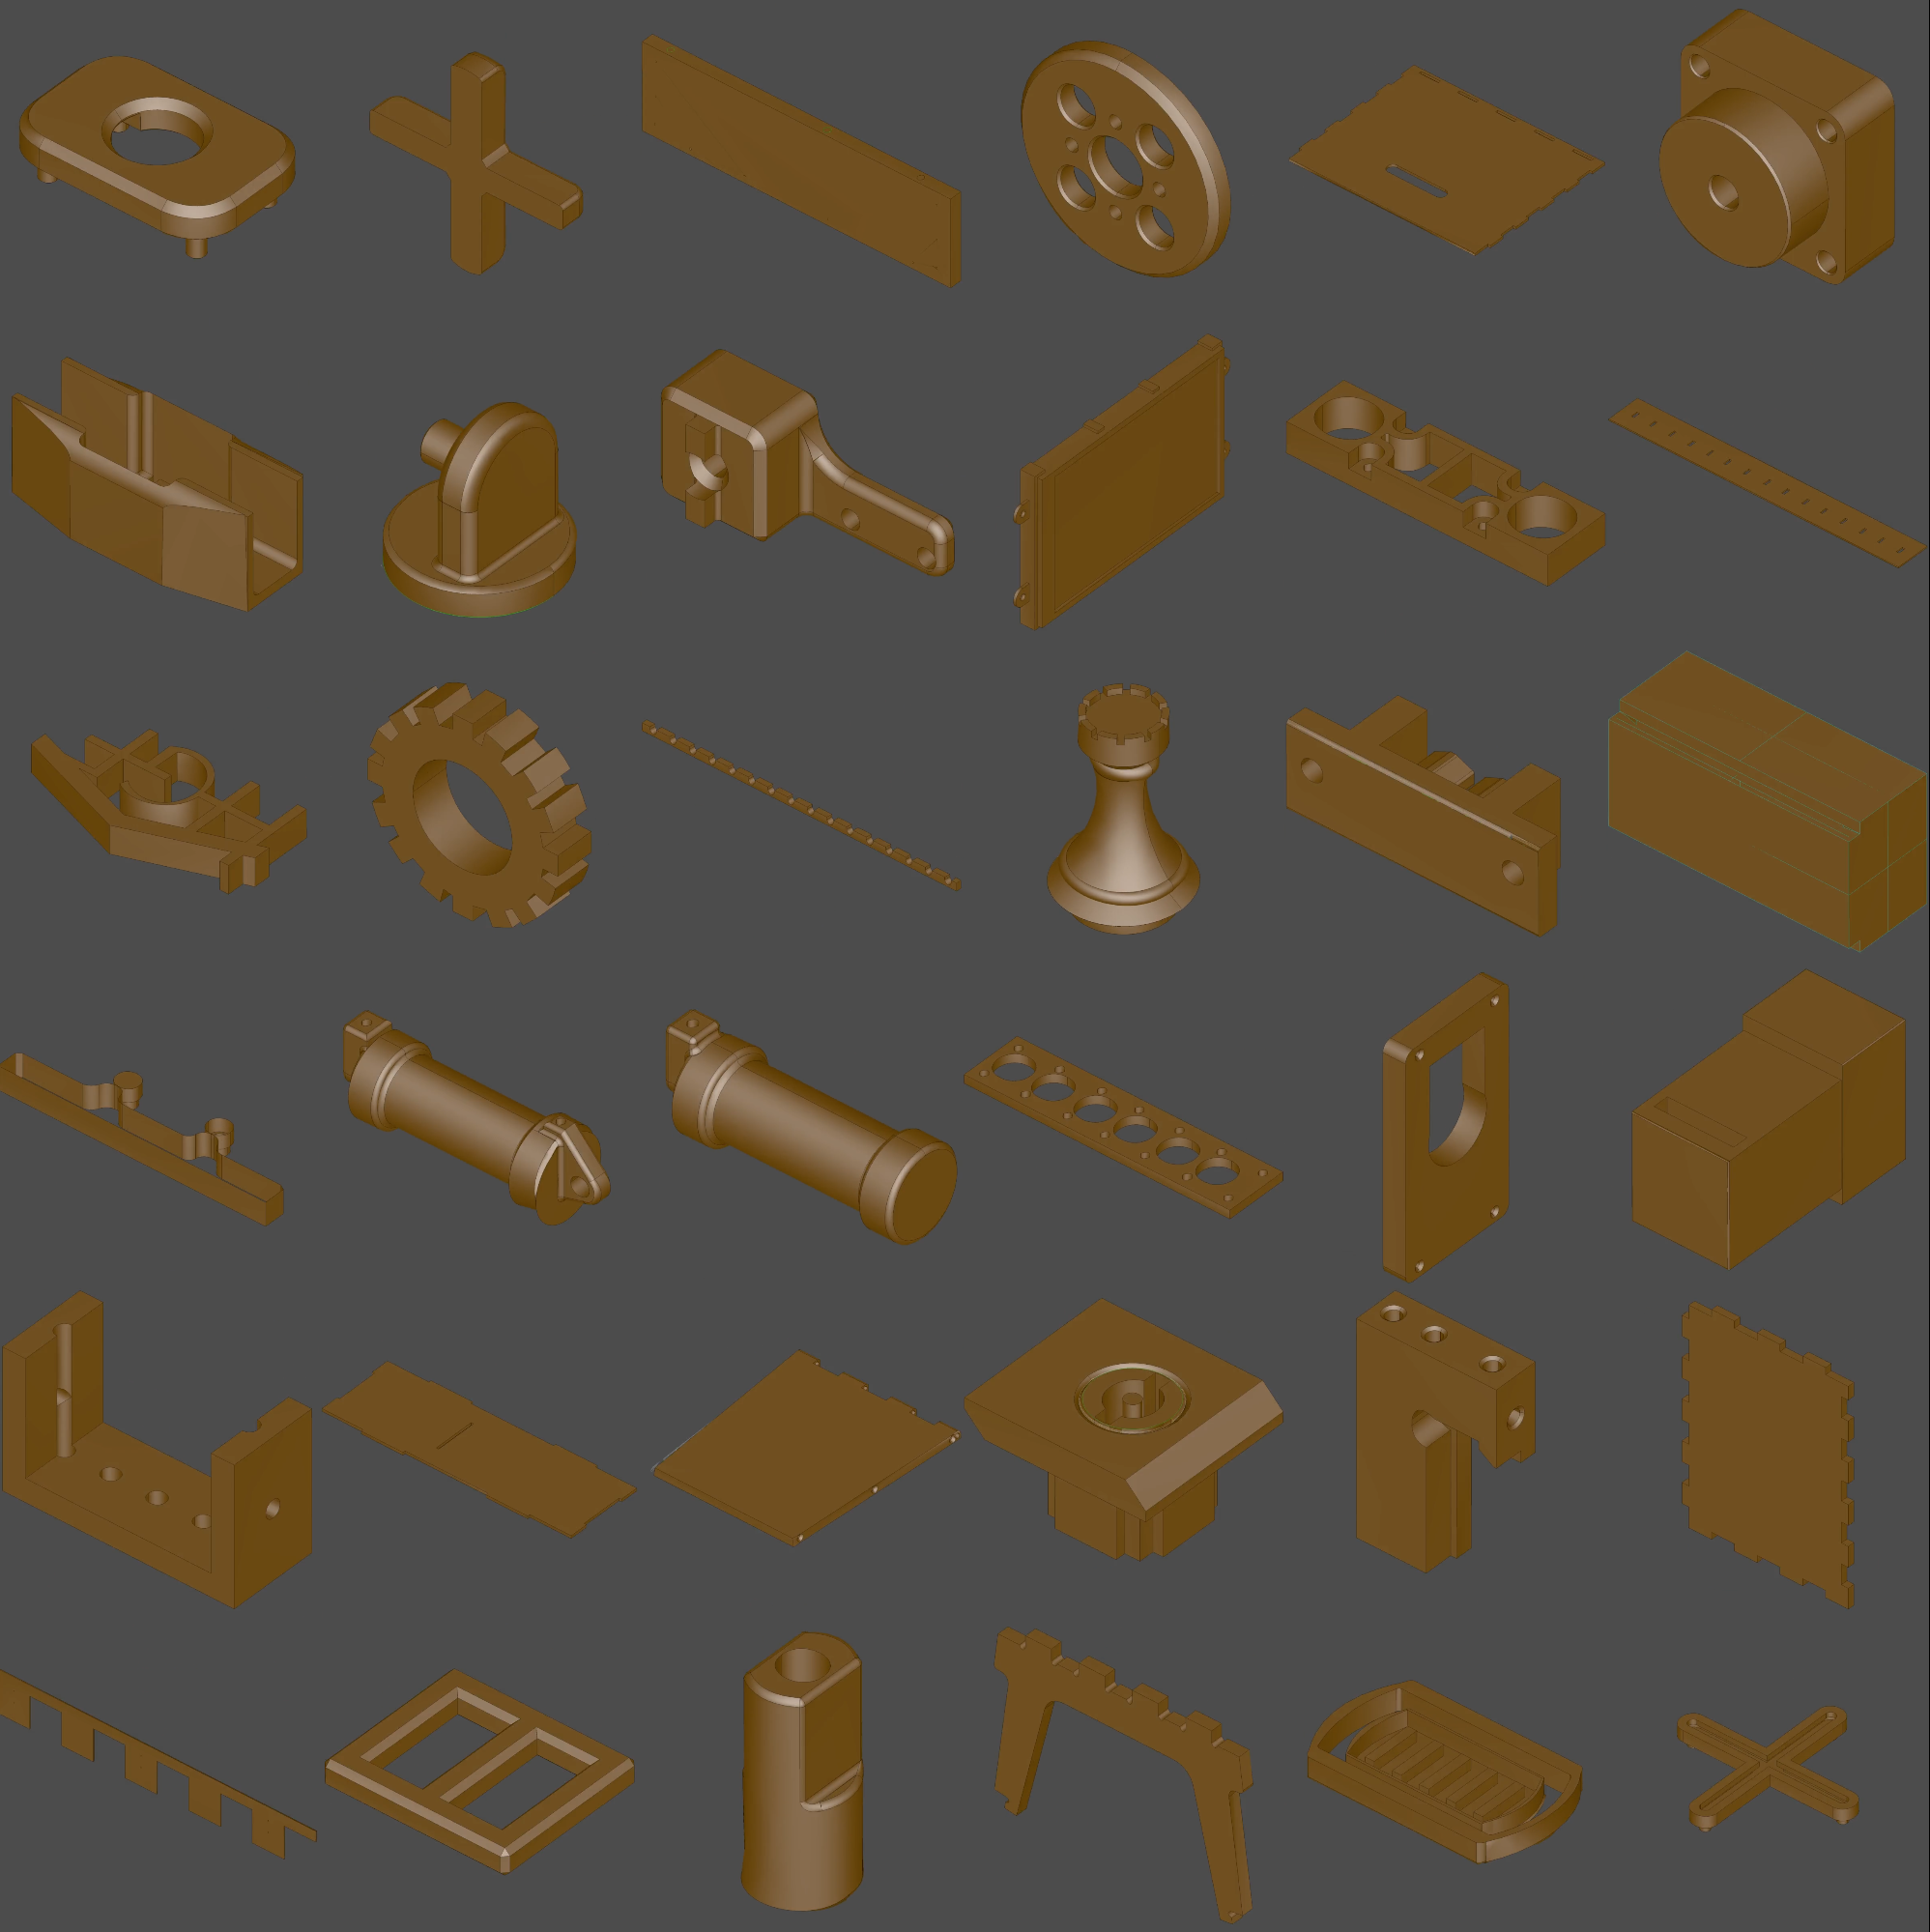
\includegraphics[width=0.66\textwidth]{figures/untuned_hard.png}
	\caption{Examples of unconditional samples generated with the untuned base model checkpoint. Top with medium complexity (25 to 50 faces per shape) and bottom with high complexity (50+ faces per shape).}
	\label{fig:untuned_samples}
\end{figure}

Generated models demonstrate:
\begin{itemize}
	\item \textbf{Geometric Validity}: Faces and edges form coherent solid structures
	\item \textbf{Diversity}: Multiple samples exhibit varied feature combinations
	\item \textbf{Domain Adherence}: Generated geometry aligns with training domain characteristics
\end{itemize}

%===============================================================
\subsubsection{Comparison with BrepGen}
%===============================================================

To contextualize AutoBrep's performance, we compare it with BrepGen, the predecessor diffusion-based approach discussed in Chapter~\ref{chap:background}. Figure~\ref{fig:brepgen_samples} shows representative samples generated with BrepGen.

\begin{figure}[h!]
	\centering
	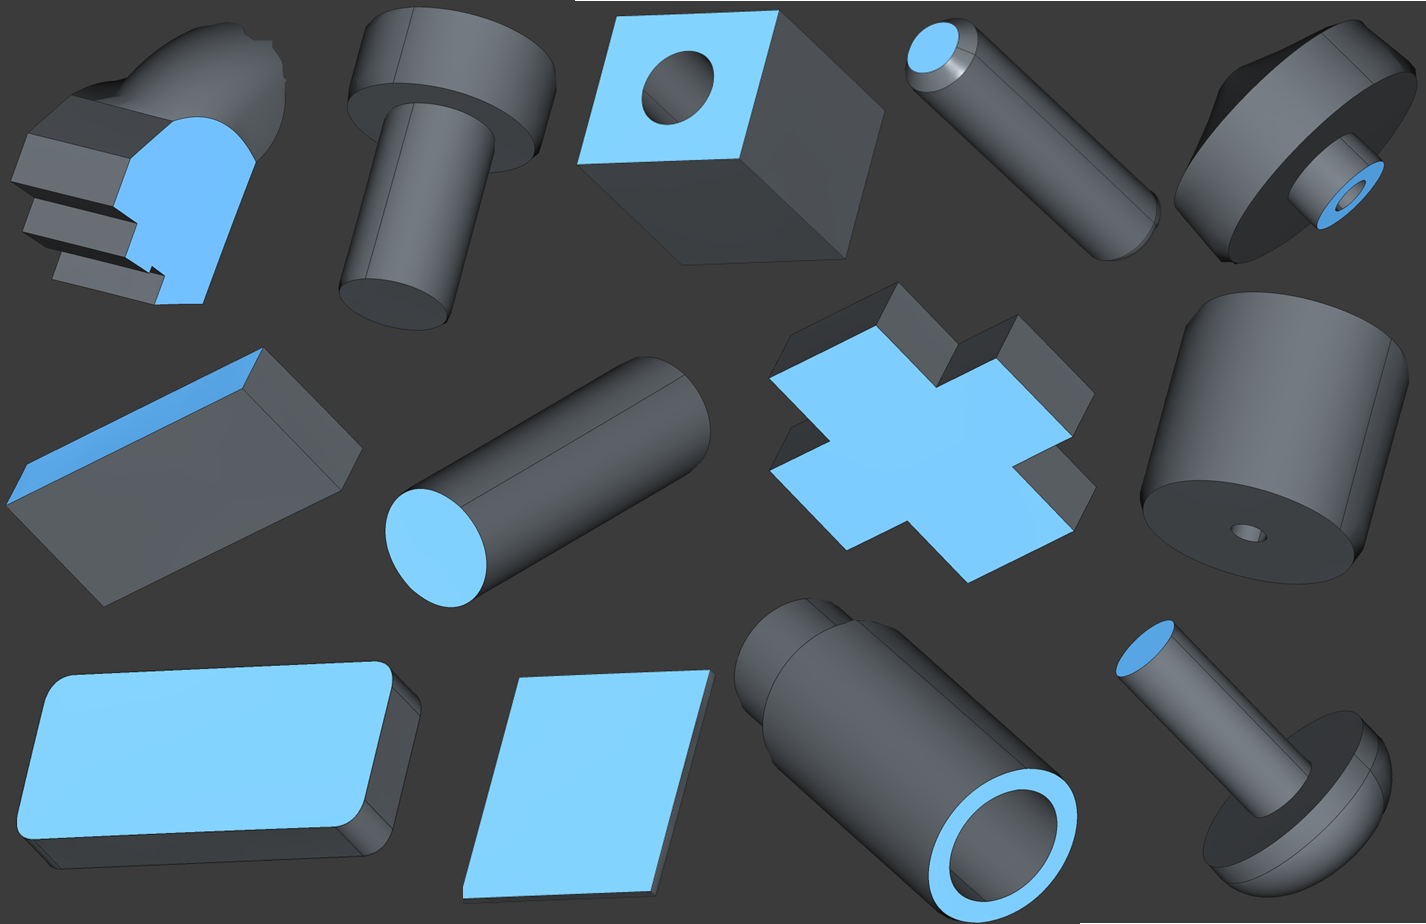
\includegraphics[width=0.66\textwidth]{figures/BrepGen.png}
	\caption{Representative samples generated with BrepGen (diffusion-based approach) from unconditional generation. While geometrically valid, BrepGen produces predominantly simple geometries with low complexity: mainly cylinders and cuboids with chamfers and holes. This limitation in generated geometric diversity motivated the selection of AutoBrep, which generates higher-complexity solids with more varied topological structures.}
	\label{fig:brepgen_samples}
\end{figure}

AutoBrep offers several key advantages over BrepGen: higher geometric complexity with diverse topological structures versus BrepGen's simple geometries (cylinders, cuboids with chamfers and holes), superior feature diversity across complexity ranges, 2--5$\times$ faster generation speed through single-stage autoregression, and better scalability supporting up to 100+ face solids.

\textbf{Base Model Constraints:} During baseline inference evaluation, we observed that the unconditionally-trained base model does not support conditional generation tasks such as autocomplete or sequence completion. The provided checkpoint appears to have been trained without geometry tokens (which are commented out in the repository code), limiting its ability to complete partial B-Rep sequences.


%===============================================================
\subsection{Training Convergence}
%===============================================================

The LoRA fine-tuning process was conducted on custom CAD model datasets, following the training setup and hyperparameters specified in Chapter~\ref{chap:methodology}.

\textbf{Training Strategy:} A key finding was that maintaining validation loss close to training loss was essential for avoiding both underfitting and overfitting. This was achieved by targeting a training loss of approximately 1.0, which empirically provided the optimal balance.

\textbf{Observed Training Characteristics:}
\begin{itemize}
	\item Training loss consistently converged toward target of 1.0 within 3--7 epochs across all datasets tested
	\item Validation loss tracked closely with training loss when hyperparameters were properly tuned (typically within 10--20\% separation)
	\item Learning rate emerged as the dominant control parameter: too high rates ($> 1 \times 10^{-4}$) caused rapid overfitting with near-zero training loss and degenerate model outputs
	\item LoRA rank and temperature had minimal influence on training convergence dynamics
	\item Gradient accumulation and bfloat16 casting proved sufficient for training on single GPU without memory issues
\end{itemize}

Training and validation loss curves are shown in Fig.~\ref{fig:training_loss}.

\begin{figure}[h!]
	\centering
	\fbox{\texttt{[Insert training/validation loss curves from W\&B export]}}
	\caption{Training and Validation Loss Over Epochs for Representative LoRA Fine-Tuning Run. Model converges toward target loss of 1.0, with validation loss tracking training loss closely.}
	\label{fig:training_loss}
\end{figure}

%===============================================================
\subsection{Empirical Findings on LoRA Fine-Tuning Dynamics}
\label{sec:lora_dynamics}
%===============================================================

\textbf{LoRA Behavior as Distribution Sharpener:} Through systematic experimentation, LoRA was observed to function as a \emph{distribution sharpener} rather than a distribution shifter. When applied to attention layers alone, LoRA concentrates probability mass on modes already present in the base model's feature space, but cannot learn genuinely novel geometric features outside this space. This fundamentally constrains what fine-tuning can achieve: the base model must already contain (in distributed form) the geometric features present in the fine-tuning data.

\textbf{Effect of Adapter Placement:} Experiments comparing attention-only adapters (as specified in Chapter~\ref{chap:methodology}, Table~\ref{tab:lora_params}) with attention + feed-forward adapters revealed minimal differences in output quality or decodability. Figure~\ref{fig:lora_adapters_comparison} illustrates the marginal improvement from adding feed-forward adapters. This finding supports the hypothesis that most adaptation occurs through attention weight redistribution, with feed-forward layers providing limited additional benefit.

\begin{figure}[h!]
	\centering
	\fbox{\texttt{[Insert comparison: attention-only LoRA vs. attention+FF LoRA at T=0.6]}}
	\caption{LoRA Adapter Configuration Comparison. Left: attention-only adapters. Right: attention + feed-forward adapters. Addition of FF adapters provides minimal visible improvement in output quality or diversity.}
	\label{fig:lora_adapters_comparison}
\end{figure}

%===============================================================
\subsection{Quantitative Evaluation}
%===============================================================

\textbf{Model Quality Metrics:} Model performance is assessed through multiple quantitative measures derived from training and inference experiments.

\textbf{Decodability Rate:} A critical metric for generative B-Rep models is the fraction of generated sequences that successfully decode into valid solids. Across all fine-tuning runs, the fine-tuned LoRA models achieved approximately 90\% decodability rate under normal inference conditions (temperature $T \in [0.5, 0.8]$). This rate remained high unless the model exhibited signs of overfitting (near-zero training loss due to excessive learning rate or epoch count), in which case generated sequences became degenerate and decoding failed completely.

\textbf{Temperature Sensitivity:} Inference temperature was varied across the range $T \in [0.3, 0.8]$ to assess its impact on output diversity and fidelity to training data. Key findings:

\begin{itemize}
	\item \textbf{Low temperature ($T \approx 0.3$)}: Model outputs concentrated on the most probable modes, with minimal diversity. Strong LoRA effect.
	\item \textbf{Optimal range ($T \in [0.5, 0.7]$)}: Best balance between resemblance to training data and geometric diversity. Results showed prominent training features (e.g., holes, cylinders, cubes) but not exact reproductions of training shapes.
	\item \textbf{High temperature ($T > 0.8$)}: Increased diversity but reduced fidelity to training distribution. Model samples from broader set of modes beyond training data.
\end{itemize}

Temperature had minimal impact on decoding success rate; failures were primarily driven by model overfitting rather than inference temperature.

\textbf{Loss Metrics:} Validation loss provided the primary signal for hyperparameter tuning. The strategy of targeting training loss $\approx 1.0$ successfully maintained reasonable separation between train and validation curves, with typical validation loss within 10--20\% of training loss for well-tuned models.

Further evaluation against baseline (untuned AutoBrep) is presented in Section~\ref{sec:ablation}.

%===============================================================
\subsection{Qualitative Results}
%===============================================================

Generated B-Reps are visualized and evaluated for geometric plausibility, feature fidelity, and diversity relative to training data.

\textbf{Cylinders with Holes Dataset:} Fine-tuning was performed on 600 cylindrical solids with through-holes. The fine-tuned model produced results featuring:

\begin{itemize}
	\item Cylindrical geometry (primary feature)
	\item Through-holes positioned and sized in plausible locations
	\item Variations in hole placement and size
	\item Decodable, watertight solids in approximately 90\% of samples
\end{itemize}

Examples are shown in Fig.~\ref{fig:cylinders_results}.

\begin{figure}[h!]
	\centering
	\fbox{\texttt{[Insert 3 representative cylinder-with-holes samples at T=0.6]}}
	\caption{Qualitative Results: Cylinders with Holes. Fine-tuned LoRA model generates cylindrical solids with through-holes. While not exact reproductions of training data, samples exhibit characteristic training features (cylindrical body, hole placement).}
	\label{fig:cylinders_results}
\end{figure}

\textbf{Cubes with Holes Dataset:} Fine-tuning was also performed on 600 cubic solids with holes, producing analogous results:

\begin{itemize}
	\item Cubic or near-cubic primary geometry
	\item Through-holes with varied placement patterns
	\item High decodability (approximately 90\%)
	\item Feature amplification without exact reproduction
\end{itemize}

Examples are shown in Fig.~\ref{fig:cubes_results}.

\begin{figure}[h!]
	\centering
	\fbox{\texttt{[Insert 3 representative cube-with-holes samples at T=0.6]}}
	\caption{Qualitative Results: Cubes with Holes. Fine-tuned LoRA model generates cubic solids with through-holes. Again demonstrating feature amplification from training data.}
	\label{fig:cubes_results}
\end{figure}

\textbf{Base Model vs. LoRA Comparison:} To isolate the effect of fine-tuning, we compare unconditional samples from the base model at temperature $T=0.6$ with fine-tuned LoRA samples at the same temperature, using the same random seed for reproducibility. Figure~\ref{fig:base_vs_lora} shows this comparison.

\begin{figure}[h!]
	\centering
	\fbox{\texttt{[Insert side-by-side base model vs. LoRA samples at T=0.6]}}
	\caption{Base Model vs. LoRA Fine-Tuning. Left: unconditional samples from base AutoBrep model. Right: samples from LoRA fine-tuned on cylinders-with-holes. Note the amplification of cylindrical features in LoRA outputs.}
	\label{fig:base_vs_lora}
\end{figure}

%===============================================================
\subsection{Ablation Studies and Hyperparameter Analysis}
\label{sec:ablation}
%===============================================================

To understand the contribution of different training and inference components, systematic ablation experiments were conducted.

\textbf{LoRA Rank Impact:} Varying LoRA rank $r \in \{16, 32\}$ showed minimal influence on final output quality or convergence behavior. Both configurations achieved similar decodability rates (approximately 90\%) and produced outputs with comparable feature amplification. This suggests that the primary bottleneck is the base model's learned feature space rather than adapter capacity.

\textbf{Learning Rate Sensitivity:} Learning rate emerged as the dominant hyperparameter. The relationship was nonlinear:
\begin{itemize}
	\item Too low ($< 1 \times 10^{-5}$): Insufficient adaptation; training loss converged slowly and remained high
	\item Optimal range ($1 \times 10^{-5}$ to $1 \times 10^{-4}$): Rapid convergence with controlled train--validation loss separation
	\item Too high ($> 1 \times 10^{-4}$): Rapid overfitting; near-zero loss achieved by memorization, producing degenerate outputs
\end{itemize}

Learning rate was therefore tuned per dataset based on validation loss monitoring.

\textbf{Temperature Impact:} Temperature variation ($T \in [0.3, 0.8]$) had negligible effect on decodability; approximately 90\% of samples remained decodable across the entire range. The effect was primarily on diversity and fidelity (see Section~\ref{sec:quantitative}).

\textbf{Comparison: Baseline vs. LoRA-Tuned:}

\begin{table}[h!]
	\centering
	\caption{Baseline vs. LoRA-Tuned Model Comparison}
	\label{tab:baseline_comparison}
	\small
	\begin{tabularx}{\textwidth}{@{}l X l l@{}}
		\toprule
		\textbf{Aspect} & \textbf{Description} & \textbf{Baseline} & \textbf{LoRA-Tuned} \\
		\midrule
		Decodability Rate & Fraction of samples decoding to valid solids & $\approx 90\%$ & $\approx 90\%$ \\
		Feature Fidelity & Adherence to domain characteristics & Broad distribution & Amplified training modes \\
		Trainable Parameters & Additional parameters required & 0 & $\approx 262$K--$852$K \\
		Training Time & Time per fine-tuning run & N/A & 1--2 hours (single GPU) \\
		Domain Specificity & Feature alignment with custom data & Baseline capabilities & Enhanced for fine-tuned domain \\
		\bottomrule
	\end{tabularx}
\end{table}

LoRA fine-tuning introduces minimal parameter overhead (less than 0.1\% of base model) while shifting output distribution toward fine-tuning data modes. Training on datasets of 600 samples converged successfully within 3--7 epochs across both geometry types, with consistent decodability rates maintained.

    % Chapter 4: Experimental Results - Training convergence, quantitative evaluation, qualitative analysis

    \section{Discussion and Limitations}
\label{chap:discussion}

%===============================================================
\subsection{Key Findings and Insights}
%===============================================================

This work demonstrates the effectiveness of LoRA-based fine-tuning for adapting a pre-trained generative CAD model to custom domains. The results reveal several important insights:

\par

\textbf{Main contributions:}
\begin{itemize}
	\item \textbf{Practical Domain Adaptation}: LoRA enables efficient fine-tuning on limited computational budgets, making generative CAD accessible to smaller research groups and organizations
	\item \textbf{Parameter Efficiency}: Achieving domain-specific performance with $\approx$1\% additional parameters relative to the base model
	\item \textbf{Transferability}: LoRA adapters are lightweight and portable, making them suitable for deployment across various systems
	\item \textbf{Reproducibility}: Systematic documentation of hyperparameters and training procedures enables reproducible results
\end{itemize}

%===============================================================
\subsection{Scalability and Transferability}
%===============================================================

The LoRA approach demonstrates promising scalability properties:

\par

\textbf{Scalability observations:}
\begin{itemize}
	\item \textbf{Multiple Adapters}: Independent LoRA adapters can be trained for different CAD domains (e.g., mechanical parts, architectural elements) with minimal overhead
	\item \textbf{Composability}: Adapter weights can be combined or interpolated for multi-domain generation
	\item \textbf{Cross-Domain Transfer}: Adapters trained on one domain may provide useful initialization or transfer benefits to related domains
\end{itemize}

\textbf{Transferability considerations:}
\begin{itemize}
	\item \textbf{Adapter Basis Models}: All adapters share the same base AutoBrep model, ensuring consistency
	\item \textbf{Domain Specificity vs. Generality}: Fine-tuning on narrow domains may reduce generalization; balancing data diversity is crucial
	\item \textbf{Task-Specific Adaptation}: Simple modifications to conditioning tokens enable task-specific behaviors without separate training
\end{itemize}

%===============================================================
\subsection{Limitations}
%===============================================================

Several practical and methodological limitations should be acknowledged:

\par

\textbf{Data Limitations:}
\begin{itemize}
	\item \textbf{Dataset Size}: Training on limited samples ($<500$ models) introduces overfitting risk; larger, diverse datasets are preferred
	\item \textbf{Data Quality}: Inconsistent STEP file formatting or incomplete geometry specifications can degrade training
	\item \textbf{Bias in Training Data}: Skewed distributions toward certain geometric features may limit diversity of outputs
\end{itemize}

\textbf{Computational and Model Limitations:}
\begin{itemize}
	\item \textbf{Sequence Length}: AutoBrep tokenization limits the complexity of generatable geometry; very complex models may exceed token limits
	\item \textbf{Precision}: Discrete tokenization introduces quantization errors; fine details may be lost compared to continuous representations
	\item \textbf{Inference Speed}: Autoregressive generation is slower than non-autoregressive methods; batch inference is essential for practical deployment
\end{itemize}

\textbf{Evaluation Limitations:}
\begin{itemize}
	\item \textbf{Limited Metrics}: Existing CAD generation metrics (e.g., Chamfer distance) may not capture perceptual or functional quality
	\item \textbf{Subjective Quality}: Assessing whether generated models are ``useful'' or ``realistic'' requires domain expert evaluation
	\item \textbf{Reproducibility}: Stochastic nature of neural models makes exact reproduction across runs difficult
\end{itemize}

%===============================================================
\subsection{Lessons Learned}
%===============================================================

The fine-tuning process revealed practical insights for practitioners:

\par

\textbf{Best practices:}
\begin{itemize}
	\item \textbf{Learning Rate Matters}: Conservative learning rates (1e-4 to 5e-5) are critical for small datasets to avoid catastrophic forgetting
	\item \textbf{Monitoring is Essential}: Real-time loss tracking via W\&B enables early detection of divergence or overfitting
	\item \textbf{LoRA Rank Selection}: Rank 8--16 provides good balance; rank $>32$ shows diminishing returns on tested domains
	\item \textbf{Data Preprocessing}: Clean, consistent STEP files are crucial; preprocessing validation saves significant debugging time
\end{itemize}

%===============================================================
\subsection{Future Research Directions}
%===============================================================

Several promising directions for future work emerge from this study:

\par

\textbf{Technical improvements:}
\begin{itemize}
	\item \textbf{Multi-Task Learning}: Joint fine-tuning on multiple domains to improve generalization
	\item \textbf{Adaptive LoRA}: Learning rank and alpha parameters as a function of layers or task
	\item \textbf{Non-Autoregressive Generation}: Exploring diffusion or flow-based models for faster inference
	\item \textbf{Hybrid Approaches}: Combining LoRA with other techniques (e.g., prefix tuning, adapters)
\end{itemize}

\textbf{Application-focused directions:}
\begin{itemize}
	\item \textbf{Interactive Design}: Integration with CAD interfaces for real-time generation feedback
	\item \textbf{Constrained Generation}: Enforcing geometric or functional constraints during generation
	\item \textbf{Inverse Design}: Generating models from functional specifications or performance requirements
	\item \textbf{User Studies}: Evaluating practical utility of generated models in professional design workflows
\end{itemize}

    % Chapter 5: Discussion - Key findings, limitations, scalability, future directions

    \section{Conclusion}
\label{chap:conclusion}

%===============================================================
\subsection{Summary of Findings}
%===============================================================

This thesis systematically investigates Low-Rank Adaptation (LoRA) for domain-specific fine-tuning of the AutoBrep generative CAD model. As demonstrated in Chapter~\ref{chap:results}, the central finding is that LoRA functions as a \emph{distribution sharpener} rather than a distribution shifter: it concentrates probability mass onto geometric modes already present in the base model's feature space rather than learning genuinely novel features. Working with 600-sample datasets of cylindrical and cubic solids with holes, fine-tuned models consistently achieved approximately 90\% decodability into valid STEP files. Detailed hyperparameter findings---including the dominant role of learning rate, the rank saturation point, and the negligible benefit of feed-forward adapters---are reported in Section~\ref{sec:ablation}.

%===============================================================
\subsection{Key Insights}
%===============================================================

Three fundamental constraints emerged from this investigation, discussed in detail in Chapter~\ref{chap:discussion}. First, the base AutoBrep checkpoint was trained unconditionally without geometry tokens, preventing arbitrary conditional generation or sequence continuation. Second, the discrete tokenization vocabulary is sufficient for smooth reconstruction but may constrain representability of specialized feature types outside the base model's training distribution. Third, and most fundamentally, LoRA adapters cannot introduce geometrically novel features: the base model must already contain the target geometric features in distributed form for effective adaptation.

These constraints explain why LoRA fine-tuning, despite its computational efficiency, remains bounded by the base model's learned feature space. On simple geometric primitives, LoRA successfully amplified characteristic training features with minimal overhead (single GPU, 0.5 hours). This effectiveness did not extend to features outside the base model's scope.

%===============================================================
\subsection{Practical and Methodological Contributions}
%===============================================================

This work establishes guidelines for practitioners attempting domain-specific fine-tuning on limited datasets. The successful adaptation of 600-sample datasets suggests this scale represents a baseline for simple geometric domains. Conservative hyperparameter selection with continuous monitoring of train–validation loss separation proved essential for avoiding overfitting. Real-time loss tracking via Weights \& Biases enabled early detection of model degradation, while periodic inference sampling during training revealed mode collapse before final convergence.

%===============================================================
\subsection{Scope and Limitations}
%===============================================================

The experiments were limited to simple geometric primitives (cylinders and cuboids with holes) on datasets of 600 samples. Generalization to more complex assemblies, irregular geometries, or larger datasets requires further investigation. The evaluation focused on decodability rates and visual similarity rather than functional metrics like manufacturability or structural validity. Additionally, this work examined only the provided AutoBrep checkpoint without retraining the base model or exploring conditional training with geometry tokens enabled, which could potentially overcome some identified architectural constraints.

%===============================================================
\subsection{Conclusion}
%===============================================================

This thesis demonstrates that LoRA enables practical, data-efficient fine-tuning of large generative CAD models. For practitioners with limited computational resources and domain-specific adaptation needs, LoRA provides a viable pathway to leverage pre-trained models without prohibitive computational costs. The identified constraints—bounded feature space, unconditional training architecture, and limited vocabulary—are not fundamental failures of LoRA but rather reflect the base model's design choices. Future work addressing these constraints through conditional retraining, larger base models and training sets, or alternative architectures could substantially expand the scope of what fine-tuning can achieve.

The methodologies, hyperparameter guidelines, and empirical findings presented in this thesis establish a foundation for continued research in parameter-efficient fine-tuning of generative CAD models. As generative AI becomes increasingly prevalent in design automation, efficient adaptation techniques will prove essential for making advanced design tools accessible across organizations and domains.

    % Chapter 6: Conclusion - Summary of contributions, practical implications, final remarks

    % Bibliography
    \pagestyle{plain}
    % Changes the page style to 'plain' for the bibliography section, typically removing headers and using simple footers.

    \clearpage
    \printbibliography
    % Prints the bibliography based on the entries in 'references.bib' and the settings defined in the preamble.

    \addcontentsline{toc}{section}{References}
    % Adds an entry titled "References" to the table of contents.

    \clearpage

    % Appendices
    \appendix
\section{Appendix}
\label{appendix}
%===============================================================
\subsection{AI Use Declaration}
To ensure transparency and uphold academic integrity, the following table outlines the artificial intelligence (AI) tools utilized during the preparation of this report. This declaration aligns with ETH Zurich's guidelines on the responsible use of AI in scientific writing.

\begin{table}[h!]
    \centering
    \caption{AI Use Declaration}
    \label{tab:ai_use_declaration}
    \begin{tabular}{@{}p{3.5cm} p{2.5cm} p{2.5cm} p{6cm}@{}}
        \toprule
        \textbf{AI-Based Tool} & \textbf{Use Case} & \textbf{Scope} & \textbf{Remarks} \\ \midrule
        GitHub Copilot Claude Haiku 4.5 \newline  & Code and table generation & boilerplate code and latex formatting & -  \\ \midrule
    \end{tabular}
\end{table}

    % Includes the content of 'appendix.tex' which should contain any supplementary material or appendices.

\end{document}
